\documentclass[12pt,twoside,letterpaper]{article}
\usepackage{graphicx}
\usepackage{amsmath}
\usepackage{float}

\begin{document}
\title{Cutting a Spur Gear on the Van Norman 16 Mill}
\author{Andrew Young}
\date{6/10/2018}


\maketitle

\begin{abstract}
This document describes the process of replicating a spur gear using a Van Norman 16 milling machine. The instructions are intended for technical students or hobbyists interested in making a replacement gear via horizontal milling.
\end{abstract}

\noindent\fbox{%
\parbox{\textwidth}{%
	
\includegraphics[width=0.5in]{exclamation}
	SAFETY WARNING: Milling machines are dangerous, and misuse can result in serious injury or death. KEEP HANDS AWAY FROM MOVING PARTS AT ALL TIMES. 
	}%
}
\noindent\fbox{%
\parbox{\textwidth}{%
	
\includegraphics[width=0.5in]{exclamation}
	PPE NECESSARY: Use eye protection at all times when working with the machine described in this manual. Wear short sleeves and well-fitting clothign that can not get caught in open machinery parts. Do not wear gloves or anything on the hands that could catch in moving parts.
	}%
}
\noindent\fbox{%
\parbox{\textwidth}{%
	
\includegraphics[width=0.5in]{exclamation}
	DISCLAIMER: The author of this manual disclaims liability for any damages caused by the use, or misuse of the information in the manual. This process involves operating a machine tool under power, and as such, there is a grave risk of personal injury if undertaken by someone who is not adequately informed, or worse, is not adequately attentive to the risks inherent in the task. 
	If you feel you are unsure of how to conduct any step in a safe, controlled manner, please go take a class from a qualified instructor, and do not rely on this manual as a sole instructive device. 
	}%
}

\clearpage

\tableofcontents

\section{Introduction}

This manual will walk you through creating a replacement gear using a Van Norman 16 milling machine, with a horizontal dividing head by the same manufacturer. The methods described herein apply specifically to straight-toothed spur gearing using the inch standard. 

\subsection{ Time Needed}

The speed of the process depends on the number of teeth to be cut and the skill of the operator. Generally, you should plan on taking your time, maybe 5 minutes per tooth starting out, plus setup and cleanup time. For a 16-tooth gear, that might be about two hours, provided all materials are at hand.


\subsection{Necessary Preparation and Background}
Please read and understand the operator manual for the mill - all relevant information for gear cutting will be included here, but you should consult the manufacturer's manual for matters such as routine lubrication and maintenance of the mill.

In addition, you will need to make or procure a cylindrical blank for cutting the gear teeth into. Determining the dimensions of the blank will be part of section \ref{sec:measuring}, but the turning of the blank on the lathe is outside of the scope of this manual.


The steps for gear replication are, broadly:

\begin{enumerate}
\item Measure the gear that is desired to be replicated
\item Machine Setup
\item Gear Cutting
\item Verifying Measurements
\item Cleanup
\end{enumerate}




\subsection{ Needed Items and Resources}

The following tools and materials will be needed to make a replacement gear. Many of the exact sizes needed for tools will depend on the gear being cut - see subsection 1 for the procedure determining how to choose cutters, arbors, and measuring tools appropriately.

Tools Needed: 

\begin{itemize}
\item Van Norman 16 Milling Machine
\item Van Norman 10in. horizontal index head and tailstock
\item Index Plate for index head
\item Standard mounting studs and nuts for mill table
\item Arbor Press
\item Mandrel for gear blank
\item Lathe Dog for Mandrel
\item Copper or brass Shim Stock
\item Cutter arbor fitting a VN 'C' taper
\item Spacers for Cutter Arbor
\item Gear Cutter
\item S.A.E Wrenches
\item Gear measuring wires
\item Micrometer of appropriate size or calipers (micrometer preferred)
\item Acid brush or coolant system
\item Dial indicator and magnetic base
\item Machinery's Handbook, 15th ed. or later
\end{itemize}


\subsubsection{Materials}

\begin{itemize}
\item Gear example to copy
\item Gear blank of appropriate size (calculate size using procedure in subsection 1)
\item Cutting oil or coolant of choice
\end{itemize}

\subsection{Cautionary Notes}

\begin{itemize}
\item Do NOT attempt to cut gearing without coolant or lubricant, with the exception of cast iron gearing. Doing so will reduce tool life significantly. 
\item Machine tools are dangerous. Observe standard shop safety procedures including wearing eye protection and hearing protection, if necessary. Keep hands away from moving parts. 
\item Read all instructions thoroughly before attempting to follow procedure. Be familiar with the operator's manual and the parts of the machine. 
\item Ensure procedure is followed carefully and double-check setups before running under power. Failure to do so may result in a machine crash and, under certain circumstances, severe injury or death.
\end{itemize}




\subsection{An Orientation to The Mill}


You should be familiarized with all basic controls of the milling machine, having read the manufacturer's instruction manual. The images from the manual pointing out the major features are reproduced here for convenience.


\begin{figure}[H]
	\centering
		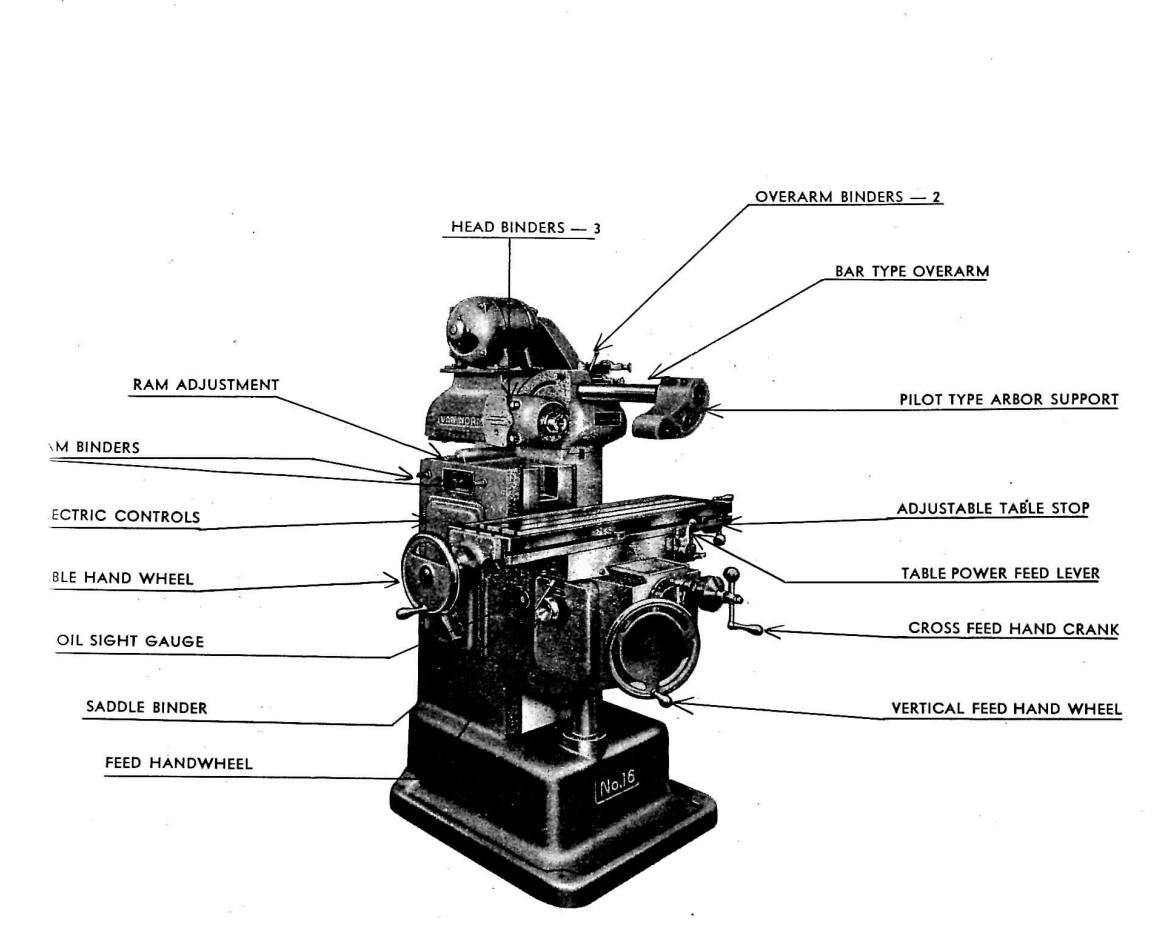
\includegraphics[width=5in]{diagram1}
\caption{Mill image 1. Adapted from ``Installation, Operation, and Maintenance Instructions and Parts List for No. 16 Van Norman Ram Type Milling Machine Plain and Universal Models'' [Pamphlet]. (1952). Springfield, MA: Van Norman Company. }
\end{figure}

\begin{figure}[H]
	\centering
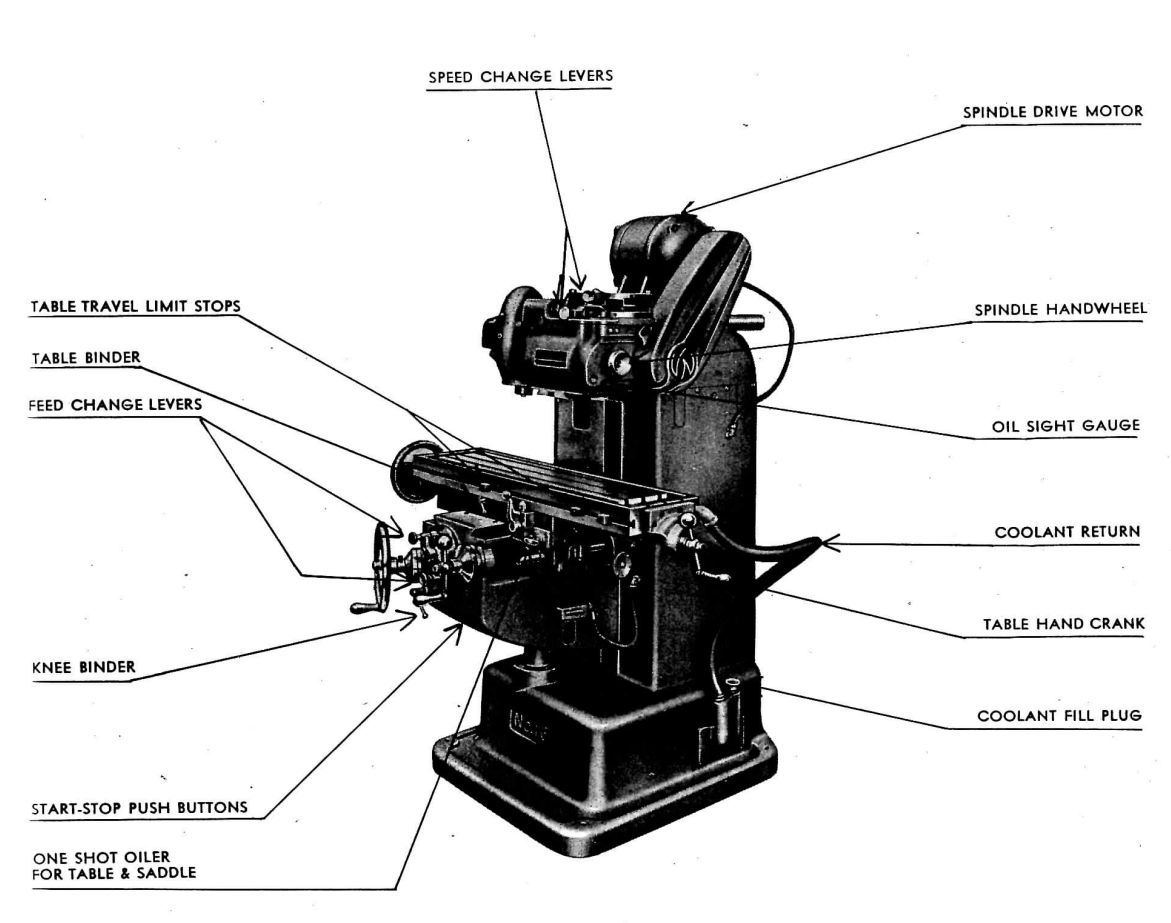
\includegraphics[width=5in]{diagram2}
\caption{Mill image 2. Adapted from ``Installation, Operation, and Maintenance Instructions and Parts List for No. 16 Van Norman Ram Type Milling Machine Plain and Universal Models'' [Pamphlet]. (1952). Springfield, MA: Van Norman Company. }
\end{figure}

\section{Measuring and Specifying the Gear}
\label{sec:measuring}


Gearing has a somewhat complicated, and very specialized set of terminology used to describe it. In this section, we will introduce some of that terminology, and then show how to use it to specify a gear to be cut.



\subsection{Introduction to Gearing Terminology}


It is helpful to think of a gear as an extension of a wheel -- in fact, watchmakers still call gears ``wheels,'' an abbreviation of ``toothed wheels.''  When two gears fit together, called meshing, there is an imaginary circle that can be drawn over each gear where it touches the teeth of the other gear or gears that it meshes with. This imaginary circle is called the \textbf{``pitch circle.''} The size of the pitch circle is called the \textbf{``pitch diameter''}, abbreviated $D$.

\begin{figure}[H]
\centering
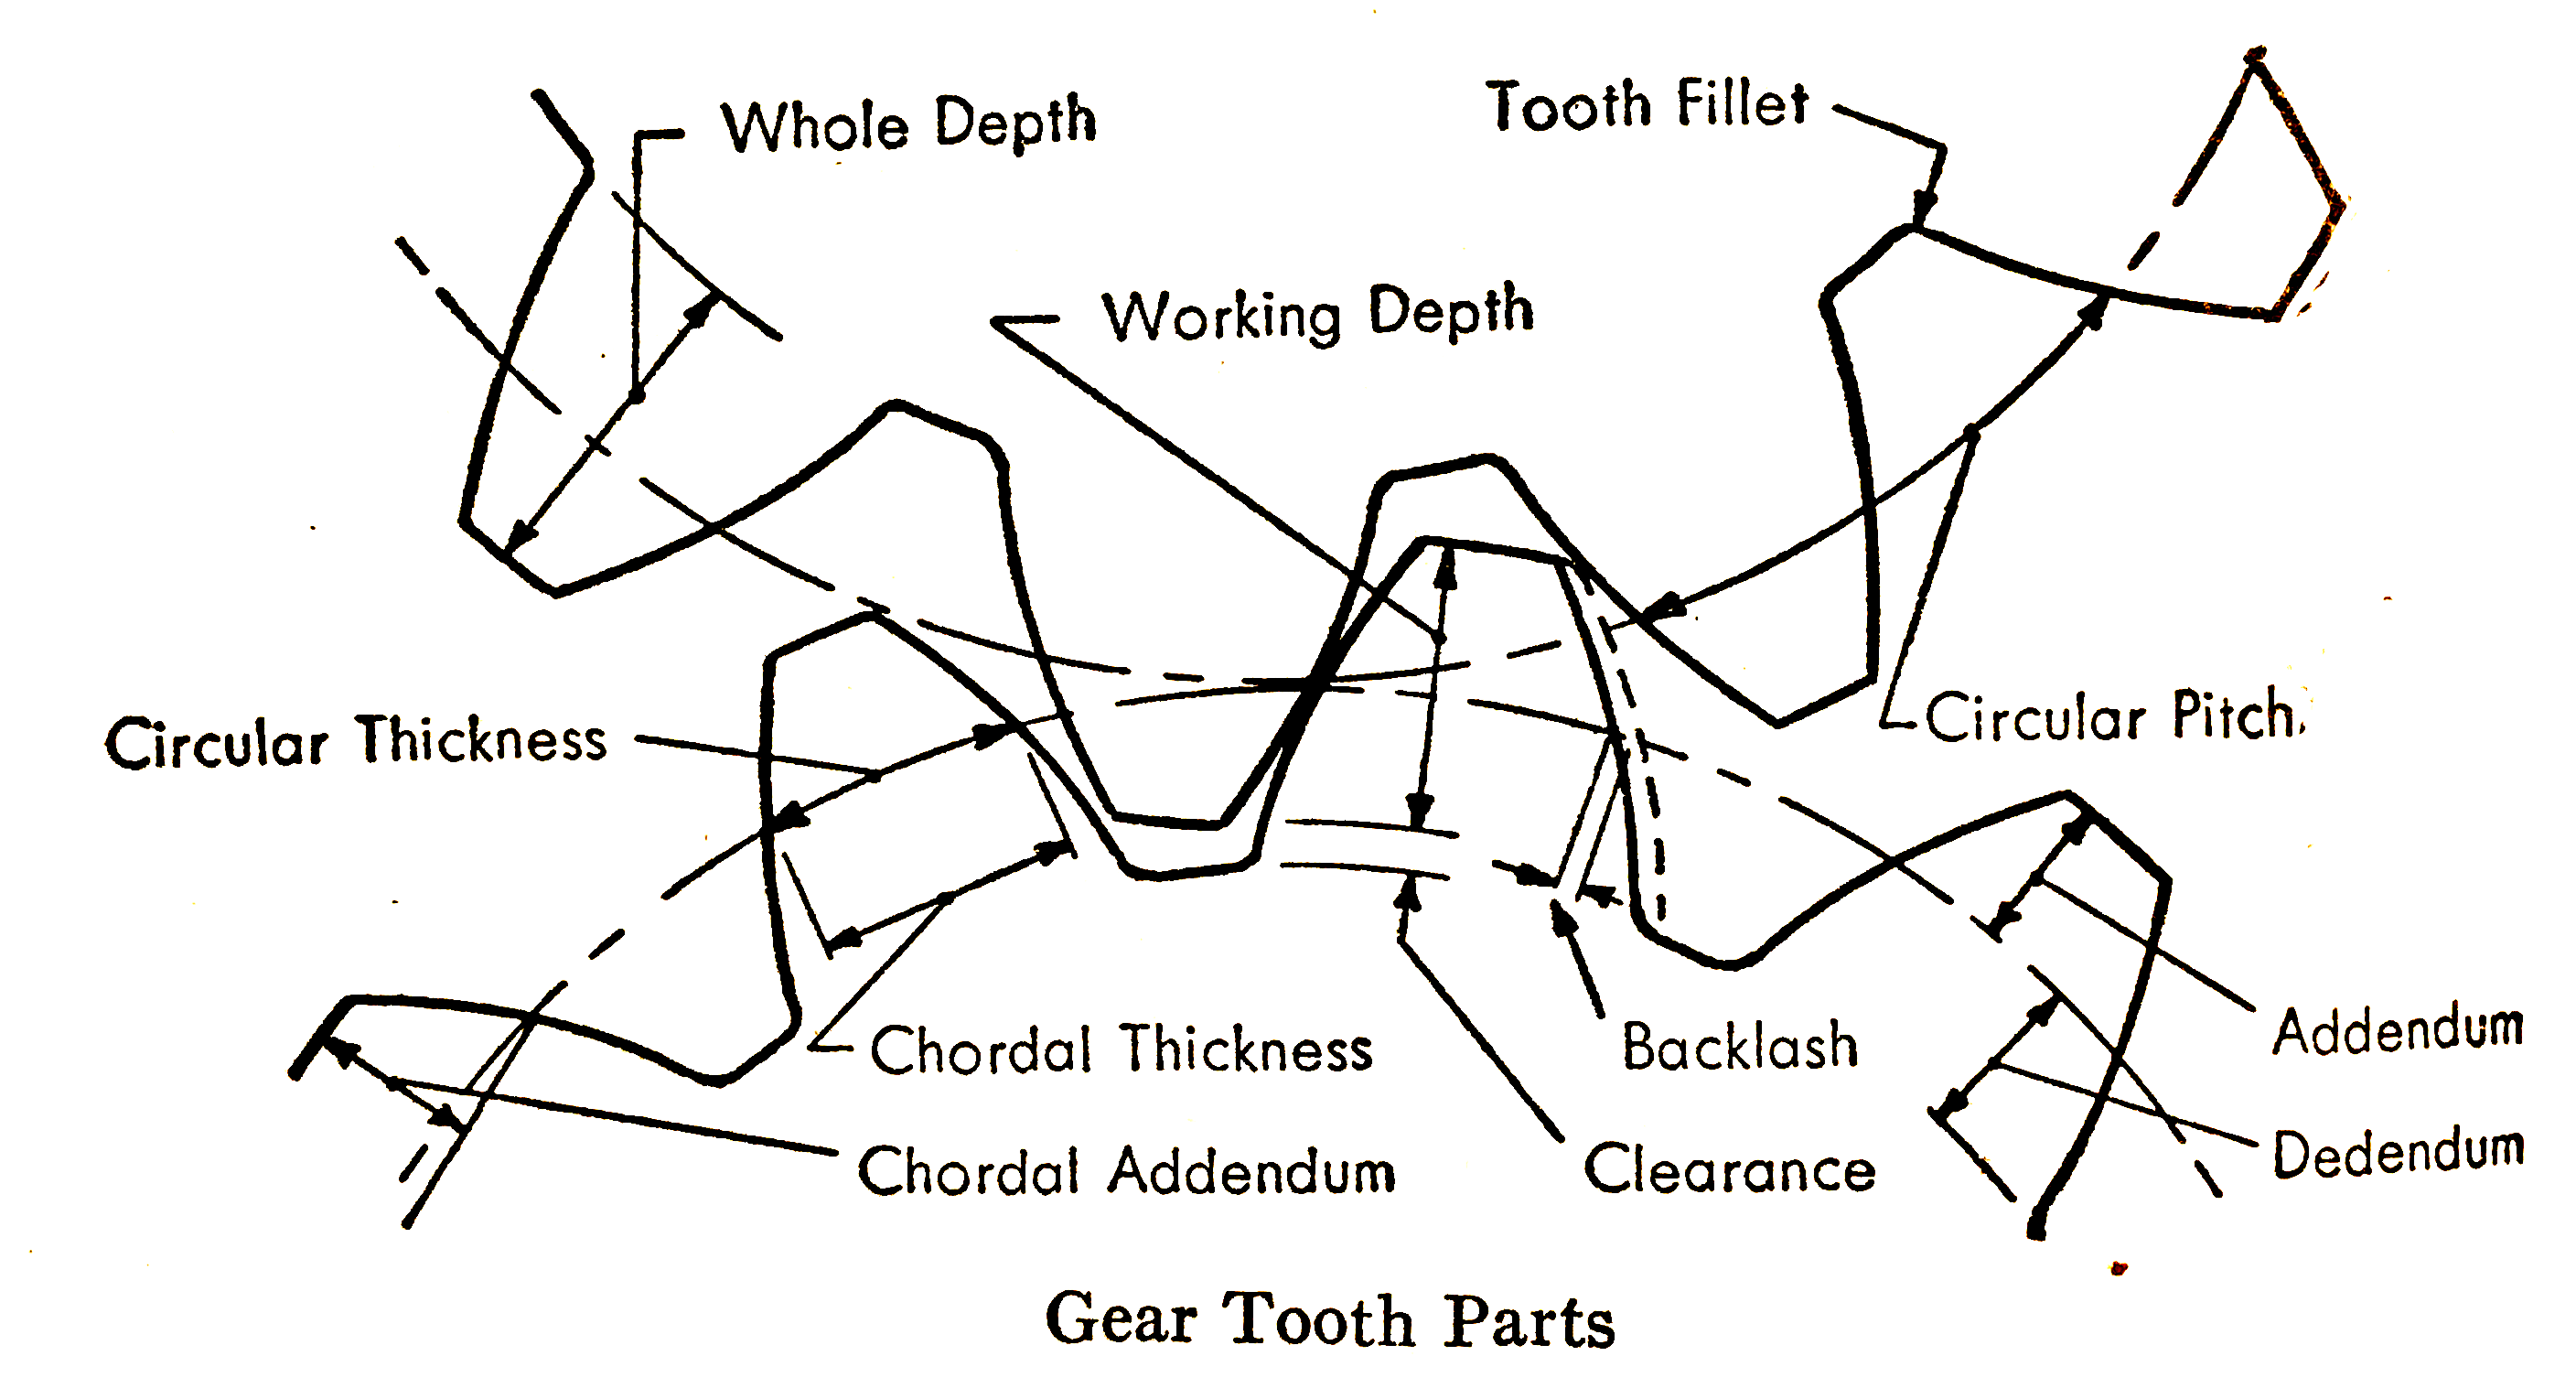
\includegraphics[width=5in]{gearparts1}
	\caption{Gear Tooth Parts. Adapted from Horton, H. L. (Ed.). (1954). Machinery's Handbook (15th ed.). New York, NY: The Industrial Press. }
	\label{fig:gearToothParts}
\end{figure}

The pitch circle acts as the reference line from which all other tooth measurements are made. Gear teeth that are compatible with each other (that will mesh at the pitch diameter) are specified as having the same \textbf{diametral pitch}, abbreviated ``$P_d$.'' The diametral pitch, the pitch diameter, and the \textbf{number of teeth,} ``$N$,'' are related using the following formula (Hinkle, 1953, p. 138):

\[P_d=\frac{N}{D}\]

When two teeth meet at the pitch circle, they do not push straight across on each other - they are designed to have an angle that they push on each other relative to the pitch circle. That angle is called the \textbf{pressure angle} (abbreviated $\phi$), so named because it is the angle, relative to a line which is tangent to the pitch circle, at which the pressure between the gear teeth is applied. The two common pressure angles for american gears are 14.5 degrees and 20 degrees.

To specify a given tooth profile (the 2D shape of the gear teeth,) these are the only three vital things to have: diametral pitch, pressure angle, and the number of teeth. 

To measure and cut a given gear, we will also use three more terms: base pitch, circular pitch, and whole depth.  The \textbf{base pitch}, abbreviated $p_b$ is the linear distance across one tooth of the gear and one gap, measured at the bottom of the tooth. The \textbf{circular pitch,} or just $p$ for short, is the linear distance between corresponding points on two teeth next to each other at the pitch circle (see Figure ~\ref{fig:gearToothParts}). The \textbf{whole depth,}  or  $h_t$, is the depth of cut necessary to carve the negative space around the tooth profiles. In regular 14.5 and 20 degree teeth, it can be calculated by: (Horton, 1954, p. 656)
 \[ h_t = 2.157 \div P_d \]


In the next section we'll introduce a procedure for finding these values from a given gear, and describe some other dimensions that need to be taken that don't affect the tooth profile, but are important for producing an identical part.


\subsection{Gathering Important Measurements}

To find the measurements for replicating the tooth profile of the gear, do the following:

\begin{enumerate}
\item Count the number of teeth on the gear, and record it as 'N'.
\item Find the outer diameter of the gear - this is the largest dimension across teeth. Record this number as `O.D.'
\item Calculate the diametral pitch, $P_d$, by the following formula:
	\[P_d  = \frac{N+2}{O.D.}\]
\item Find the pressure angle $\phi$ using the following procedure, suggested by Suvo of ``bright hub engineering,'' (Suvo, 2010)
	\begin{enumerate}
		\item Measure the distance across two gear teeth.
		\item Measure the distance across three gear teeth.
		\item Subtract the first measurement from the second to find the base pitch.
		\item Repeat the procedure several times and take the average as the final base pitch estimate.
		\item Calculate the circular pitch using the following formula: (Hinkle, 1953, p. 138)
			\[p = \frac{\pi}{P_d}\]
		\item Use the following formula to calculate the pressure angle from the base pitch and circular pitch: (Hinkle, 1953, p. 143)
			\[\phi = acos(\frac{P_b}{P})\]
	\end{enumerate}
\item Calculate the whole depth, $h_t$, by the following formula:
  \[ h_t = 2.157 \div P_d \]
\end{enumerate}

In addition to recording the important tooth measurements, also take the following measurements:
\begin{enumerate}
	\item Measure the thickness of the gear.
	\item Measure the bore of the gear.
	\item Measure the width and depth of any keyway that has been cut in the gear.
	\item Take note of any other features, such as bosses, arms, or undercut sections that may need to be replicated.
\end{enumerate}



\subsection{Using Gear Wires}
\begin{figure}[H]
	\centering
	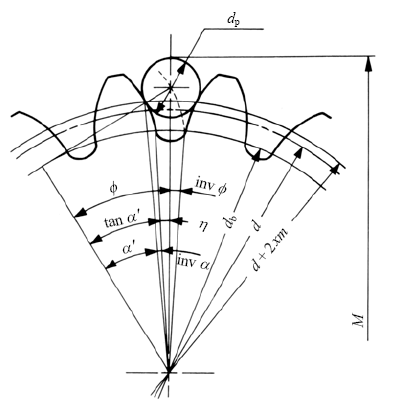
\includegraphics[width=3in]{gearInspEngEdge}
	\caption{A gear wire sitting between teeth, on the pitch circle. Adapted from Engineer's Edge, llc. (n.d.). Inspection Methods for Spur Gears | Single Pin Measurement Method. Retrieved from https://www.engineersedge.com/gears/gear\_size\_inspection.htm }
\end{figure}

When cutting gear teeth, it is important to be able to check your work. One of the simplest and best ways to measure gear teeth being cut is a set of gear wires. Gear wires are cylinders sized to sit right on the pitch diameter of the gear, to measure it indirectly. The size of a gear wire should be about 1.728 divided by the diametral pitch of the gear (Horton, 1954, p. 845) 

There are pre-made gear wires according to a standard developed by the Van Keuren company. In our case we are cutting a 16dp gear, which should use a wire of 0.10800 diameter. (Horton, 1954, p. 854)  If ground and hardened pins are not available, you may make your own, though more approximate results are to be expected. 

The actual dimension of the gear across the wires may be found by consulting Machinery's Handbook - the tables are too extensive to reproduce here.


\begin{figure}[H]
	\centering
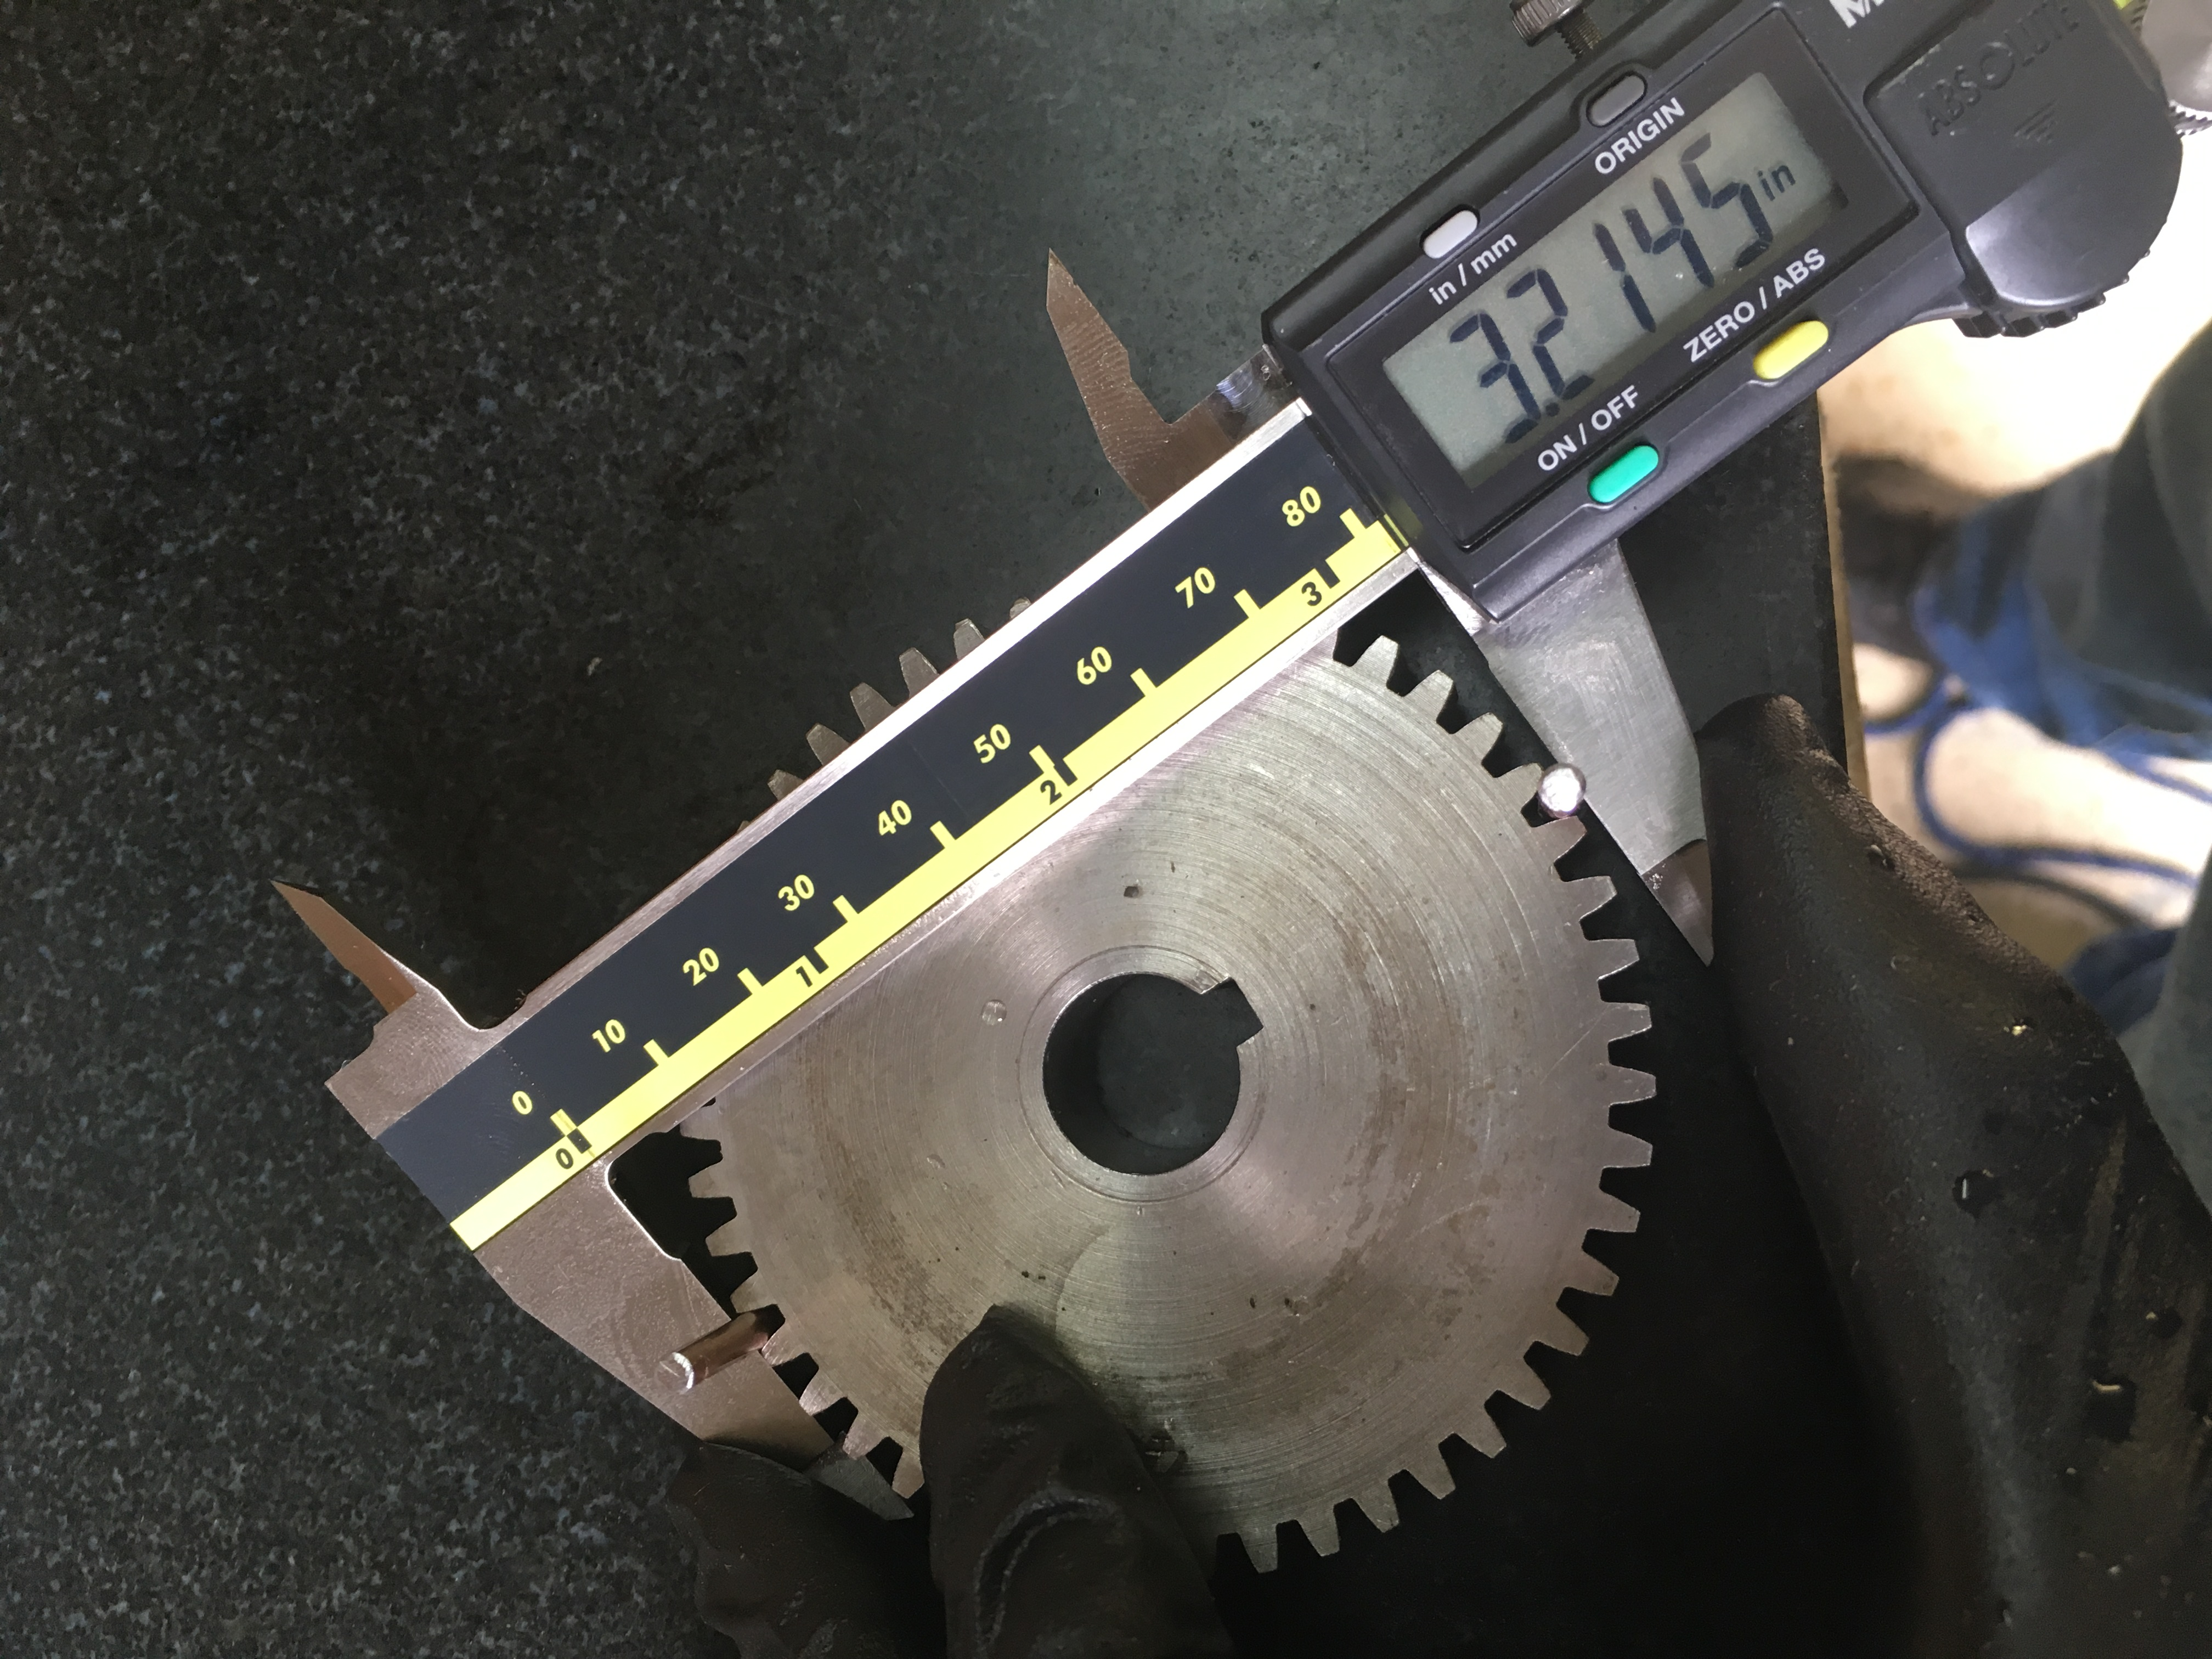
\includegraphics[width=5in]{gearMeasure}
	\caption{Measuring a gear for tooth depth, using wires. Ideally an appropriately sized micrometer would be used to minimize error, but a hobby shop can get by the careful use of a set of calipers, as pictured.}
\end{figure}

\clearpage

 
\clearpage
\section{Machine Setup}
Machine setup is key to the gear cutting process going well.  In this section, we actually start the gear manufacturing process by setting up the machine to make the necessary cuts.



\subsection{Setting up the Index}
\begin{figure}[H]
\centering
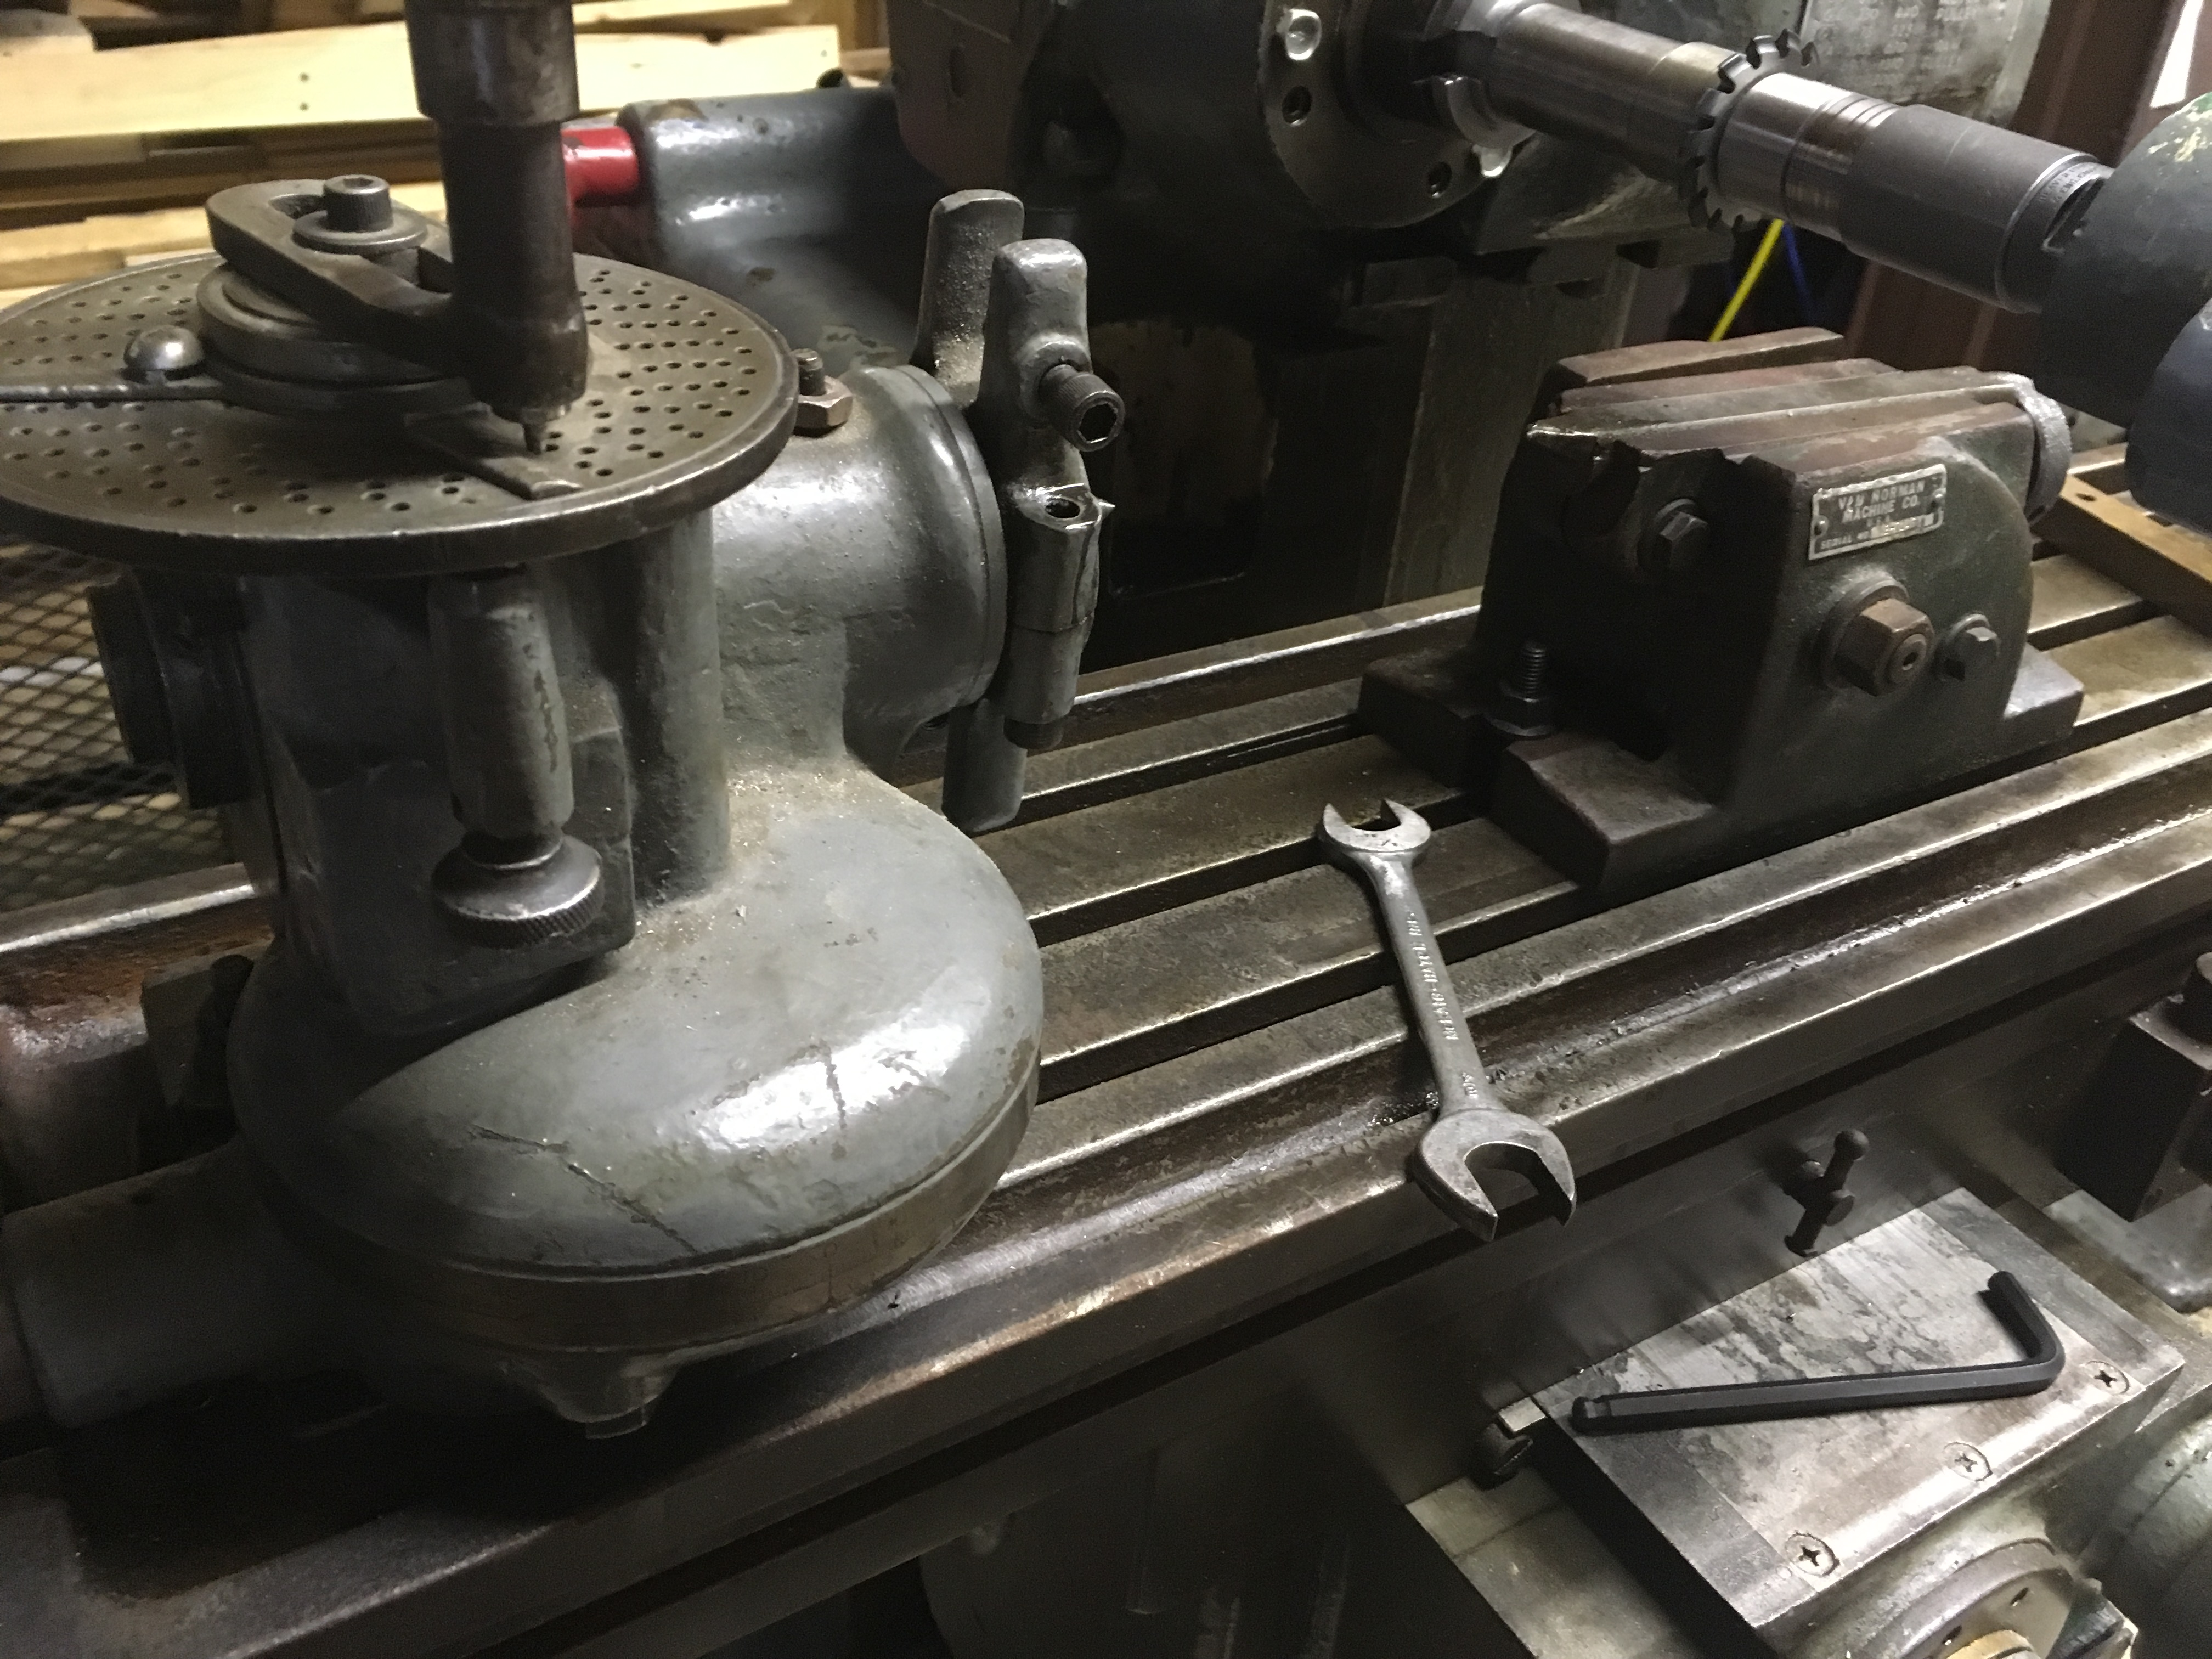
\includegraphics[width=5in]{indexOnMill}
	\caption{The Rotary Index, mounted on the mill table.}
\end{figure}

\begin{enumerate}
	\item Place the 10 inch horizontal index and the tailstock on the mill table, with the index to the left. 
	\item Ensure that the index is equipped with a dog driver and dead center.
	\item Align the index and tailstock by eye, and clamp lightly to the table using standard mounting studs.

\subsubsection{Alignment}
\begin{figure}[H]
\centering
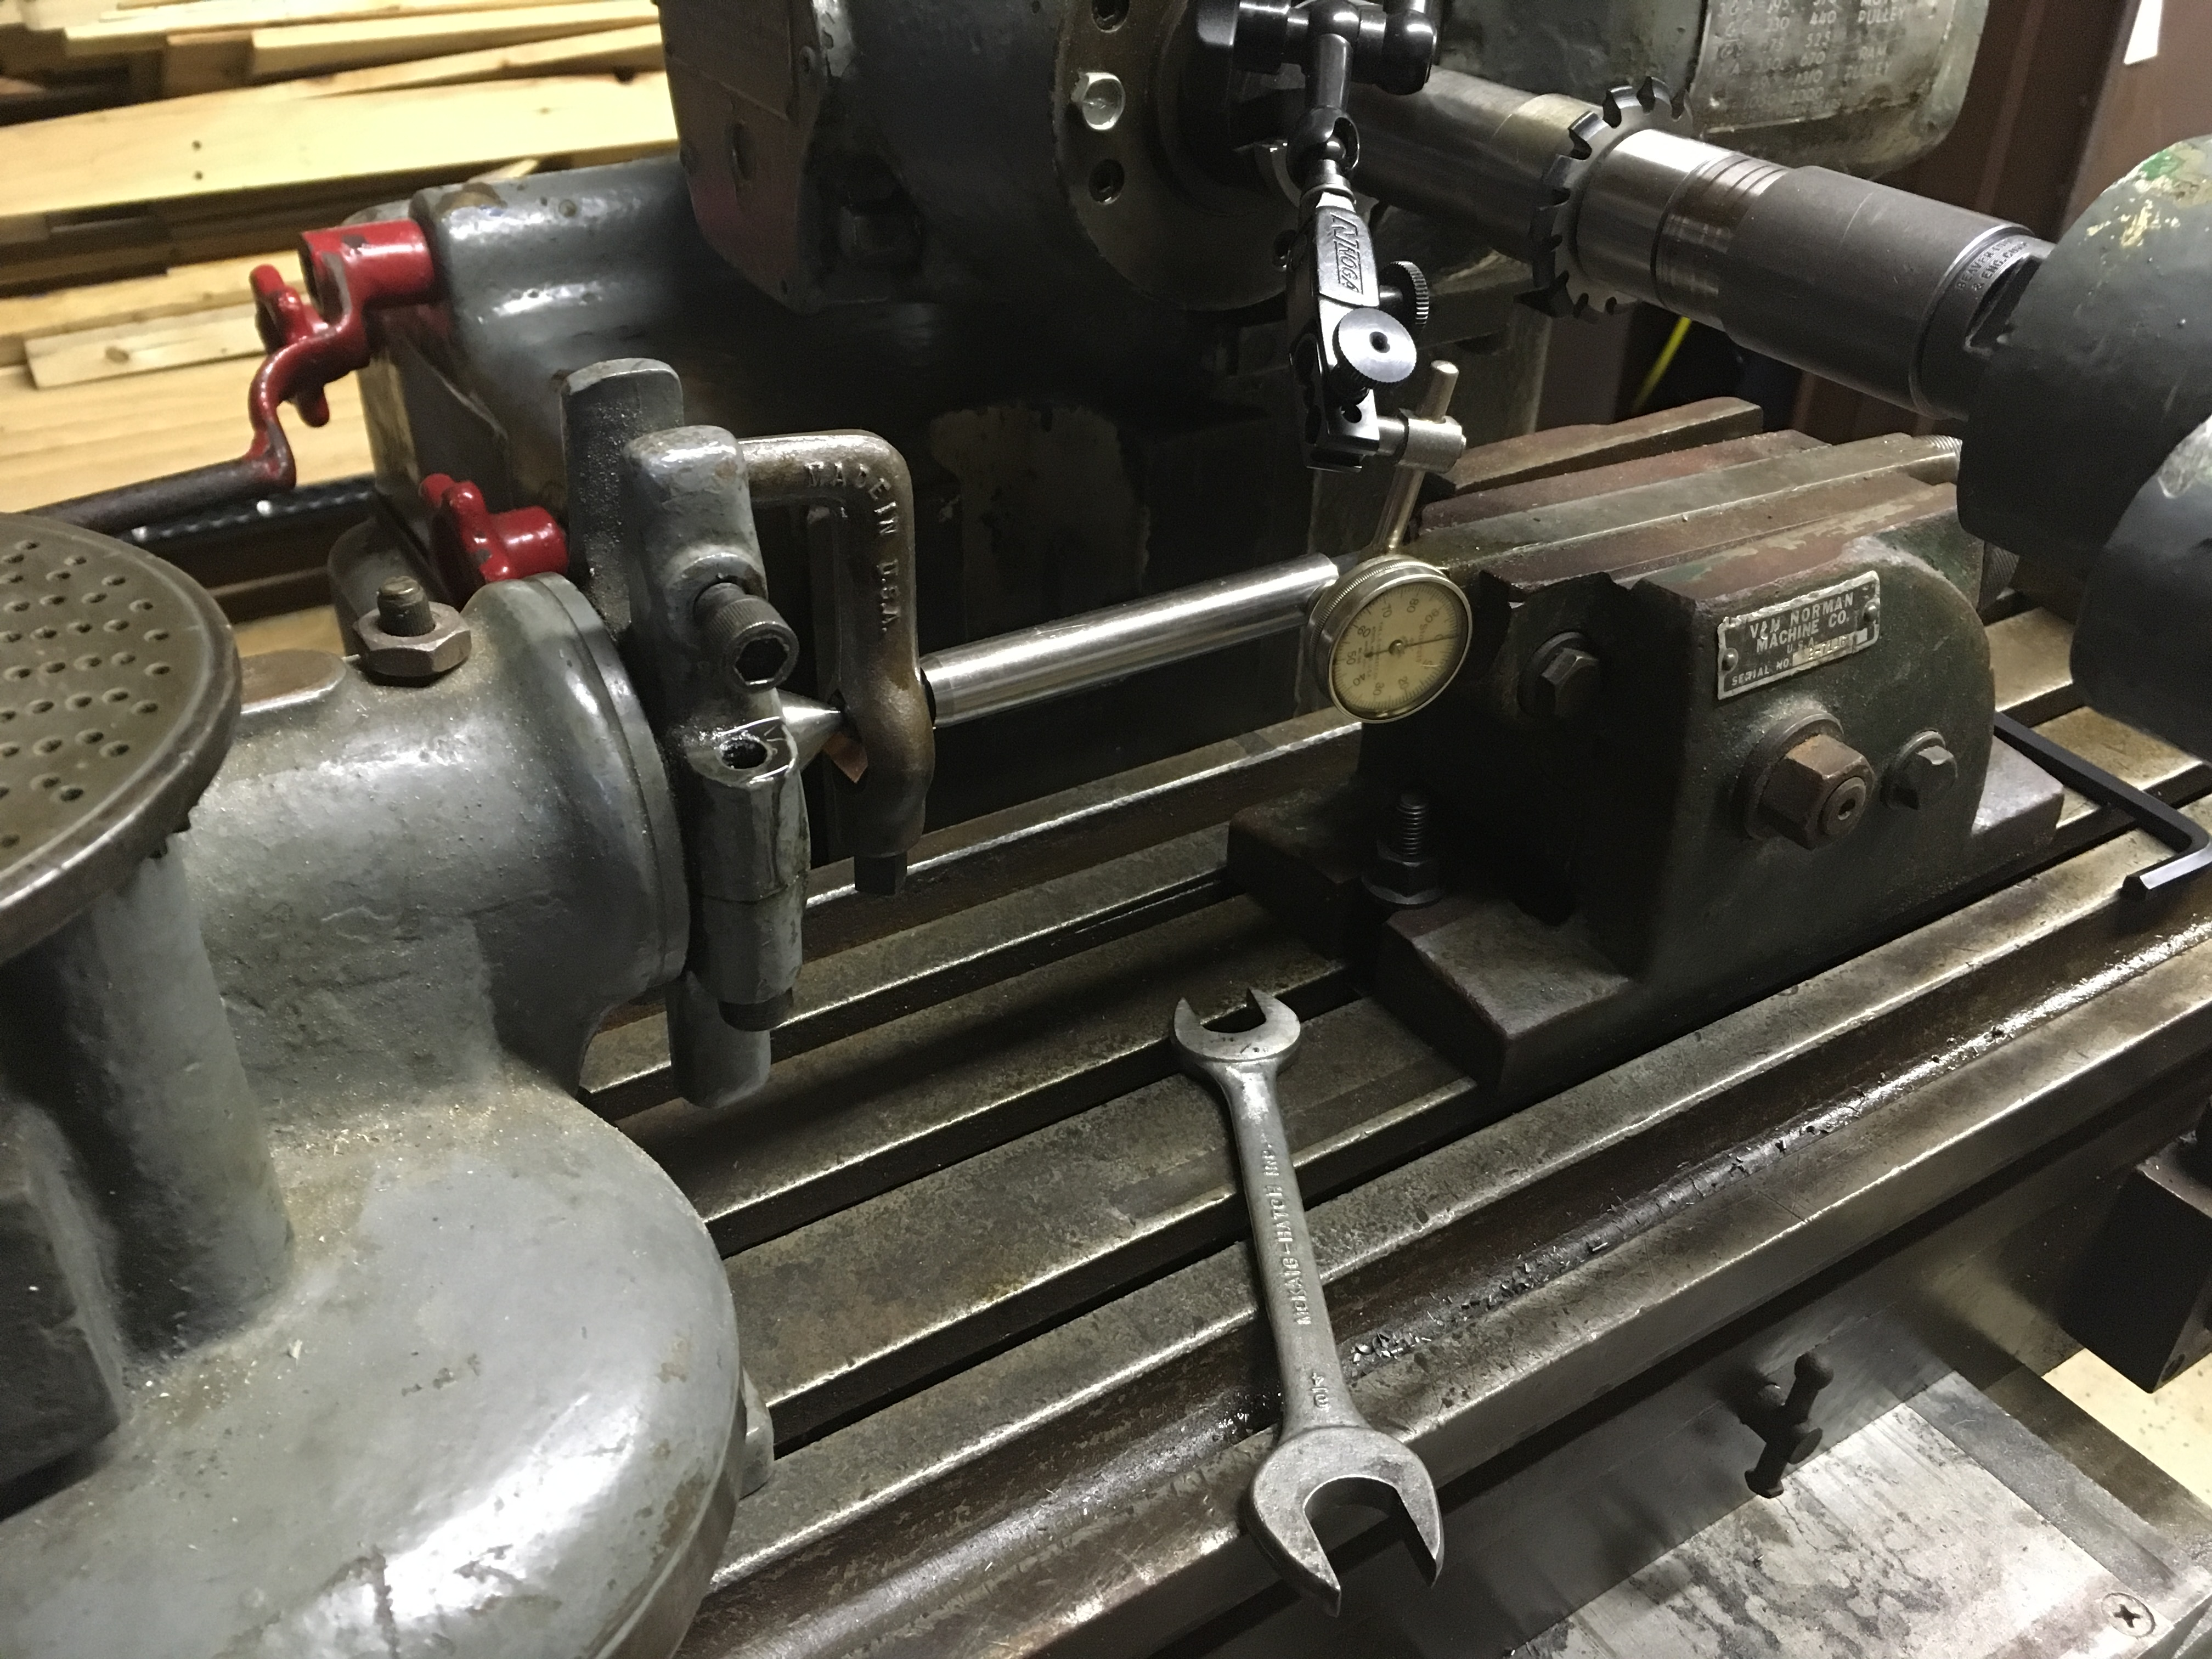
\includegraphics[width=5in]{indexSetup}
	\caption{Aligning the index centers using a dial indicator.}
\end{figure}

	\item Set the gear mandrel between centers for machine alignment. 
	\item Set a dial indicator in a magnetic base on the ram of the machine, and align it so that it can be sweep across the top of the mandrel via the table feed. 
	\item Adjust the tip of the dial indicator so that it is in contact with the top of the mandrel.
		\clearpage
	\item Sweep the indicator across the mandrel using the table feed. The indicator should show less than a thousandth difference in height. If the mandrel is tapered, keep that taper in mind when sweeping measurements across it - the change in the indication should match the taper of the mandrel if it is parallell with the axis of table travel. If the indicator shows a lack of paralellism with the table, adjust the vertical angle of the tailstock, and repeat the indicating procedure until the indicator reads that the mandrel is parallel in the vertical plane.

	\item Adjust the dial indicator so that its tip rides along either side of the mandrel (but be sure you can read the dial.)
	\item Sweep the dial indicator across the mandrel using the table feed, to verify horizontal alignment of the centers. When traversed across the mandrel by using the table feed, it should show less than a thousandth deviation from parallel. If the alignment is off, ensure that one of the bolts mounting the tailstock to the table is partially loosened, and tap the side of the tailstock with a brass drift or lead hammer until the indicator reads parallel when swept along the length of the mandrel. Again, be sure to account for any taper in the mandrel. 

	\item When alignment is correct, clamp the tailstock firmly to the table.
\subsubsection{Indexing Setup}
\begin{figure}[H]
\centering
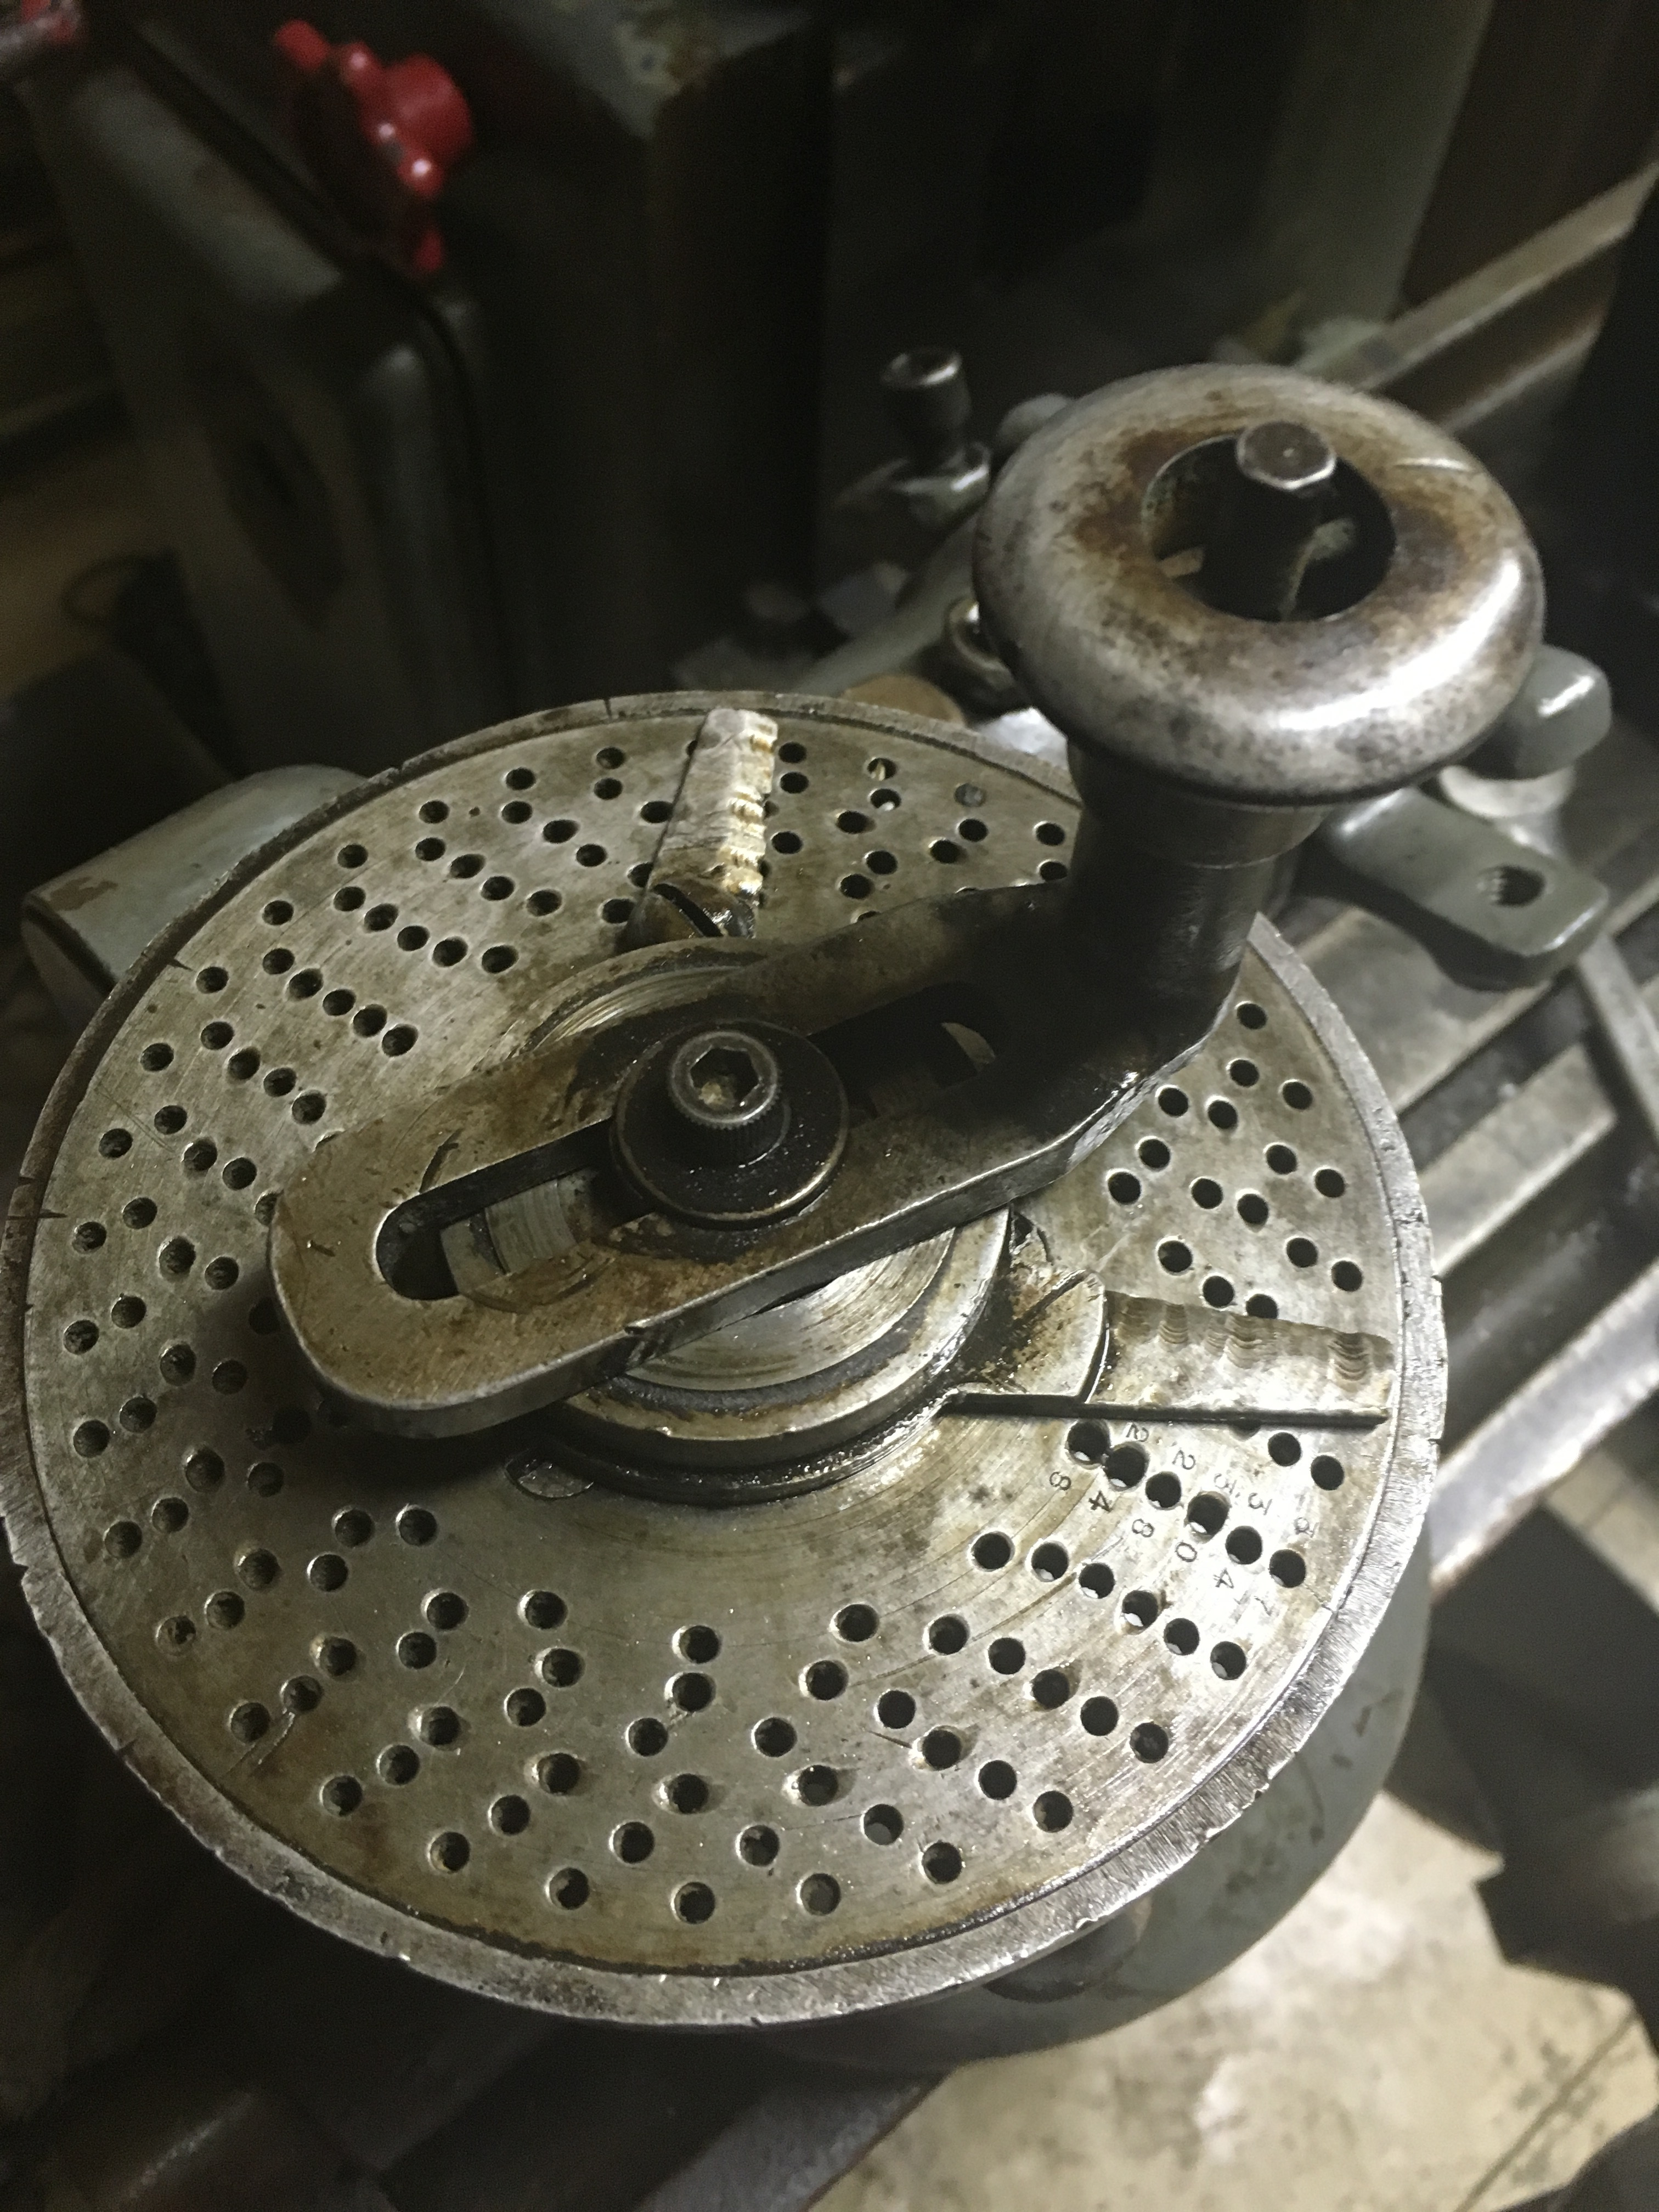
\includegraphics[width=5in]{indexPlate}
	\caption{The top of the index, showing the hole plate, the sector arms, and the worm handle.}
\end{figure}
	\item Calculate the number of turns of the index worm necessary for each gear tooth. The index worm on the Van Norman index head requires 40 revolutions of the worm (that is, of the handle on top of the index) for one full turn of the workpiece. Therefore, to calculate the number of turns for just one tooth of a 24 tooth gear:
		\[ \frac{40 turns}{24 teeth} = 1\; 2/3 \;turns/tooth \]
	\item Take the remainder of the fraction, if any, and determine if there are any hole patterns that are evenly divisible by the denominator. Choose the most convenient hole pattern that is divisible by that number.
	\item Multiply the hole pattern count by the denominator of the remainder of the turn count. This gives us the number of holes we need to advance in order to get that exact remainder of rotation In this case,
		\[ 2/3 turn \times 24 holes/turn = 16 holes \]
	\item Loosen the bolt affixing the worm-handle to the top of the index.
	\item Lift the worm handle, pulling the pin out of whichever hole it was in previously.
	\item Place the pin in one of the holes in the appropriate hole pattern (in the case of the 24-tooth gear, the 24-hole pattern was chosen.)
	\item Tighten the bolt to affix the handle to the worm.
	\item Loosen the screw holding the two sector arms together.
	\item Place one of the sector arms just counterclockwise of the pin of the worm handle.
	\item Move the other sector arm in a way that the determined hole count (16 in the example case) is exposed along the given hole-pattern. This acts as a stop to let the operator go the appropriate number of holes without counting them each time.
	\item Tighten the screw affixing the two sector arms to each other. They should now stay in the same angular relationship to one another, but still be able to be moved freely around the axis of the worm handle.
\end{enumerate}



\subsection{Setting up the Gear Blank}

\begin{figure}[H]
\centering
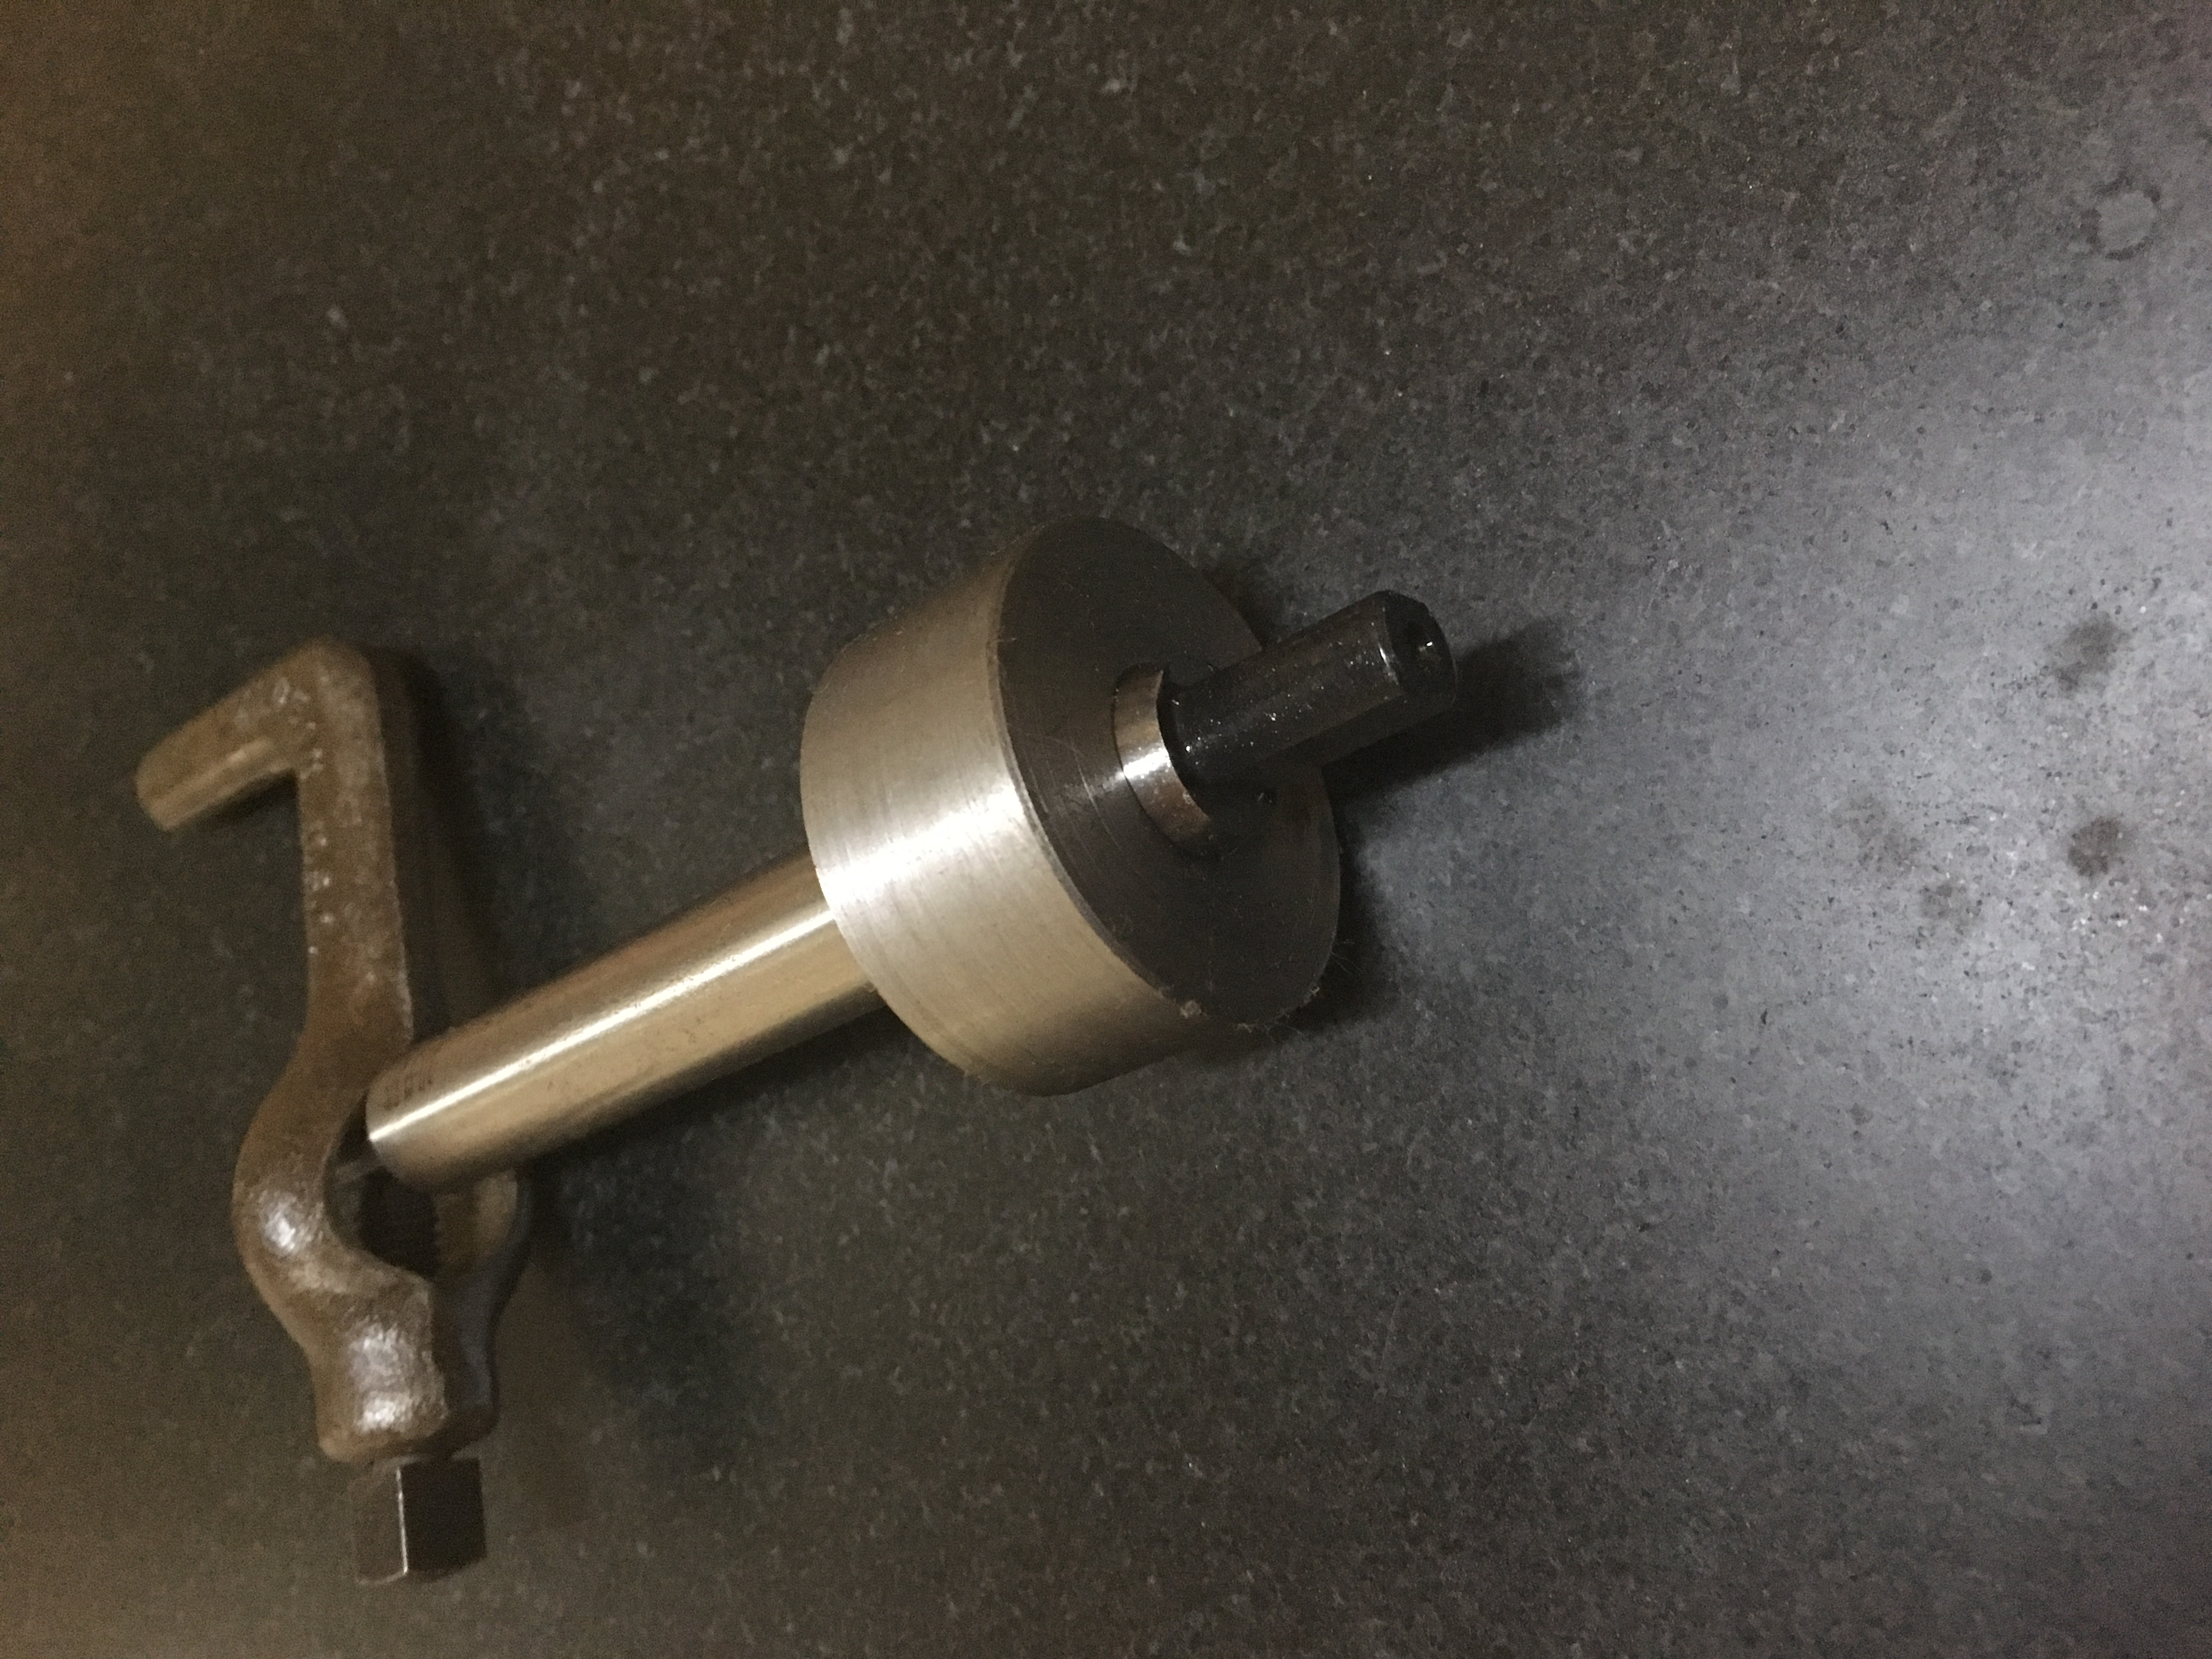
\includegraphics[width=5in]{gearBlank}
	\caption{Mounted gear blank for example project. The components of the assembly are, from left to right: lathe dog, mandrel, and gear blank.}

\end{figure}
		Making the gear blank is beyond the scope of this manual, but should fall well within the expertise of anyone familiar with lathe work. The keyway is an important part, which may be broached, filed, or shaped, depending on the materials at hand. Tolerances required for gear blanks are fairly tight - for a run-of-the-mill part, one or two thousandths maximum should be held on the main bore of the blank. If a particularly good class of work is desired, Machinery's handbook has the relevant tolerances in tabular form (Horton, 1954).

		One good way to ensure this kind of accuracy is to get some stock bored out carefully, to press it on an arbor, and then machine it to size between centers, on the arbor. This is the method used for the example gear. Once you have a gear blank, you can follow the following steps to put it in the machine:

\begin{enumerate}
	\item Remove the mandrel from the index by loosening the screw on the tailstock.
	\item Place the gear blank on the arbor. Use an arbor press to ensure the arbor is tightly fit into the bore of the gear. If a screw-type arbor is to be used instead, tighten it firmly.
	\item Place lathe dog and copper shim on arbor, and tighten the dog. Be sure to use the copper shim to prevent marring the outside of the arbor.
	\item Tighten the lathe dog in place using a wrench.
	\item Place mandrel back between centers and mount snugly, using tailstock screw to cinch up on arbor. Ensure that the tail of the dog is in the dog driver plate.
	\item Tighten the screw on the dog driver plate to ensure the setup does not come loose. This secures the workpiece from axial rotation.
	\item Tighten the bolt on the tailstock center to ensure that it does not back out of the holes mid-cut. This secures the workpiece in all rectilinear axes of motion.
\end{enumerate}


\subsection{Setting up the Cutter Arbor}
\begin{figure}[H]
\centering
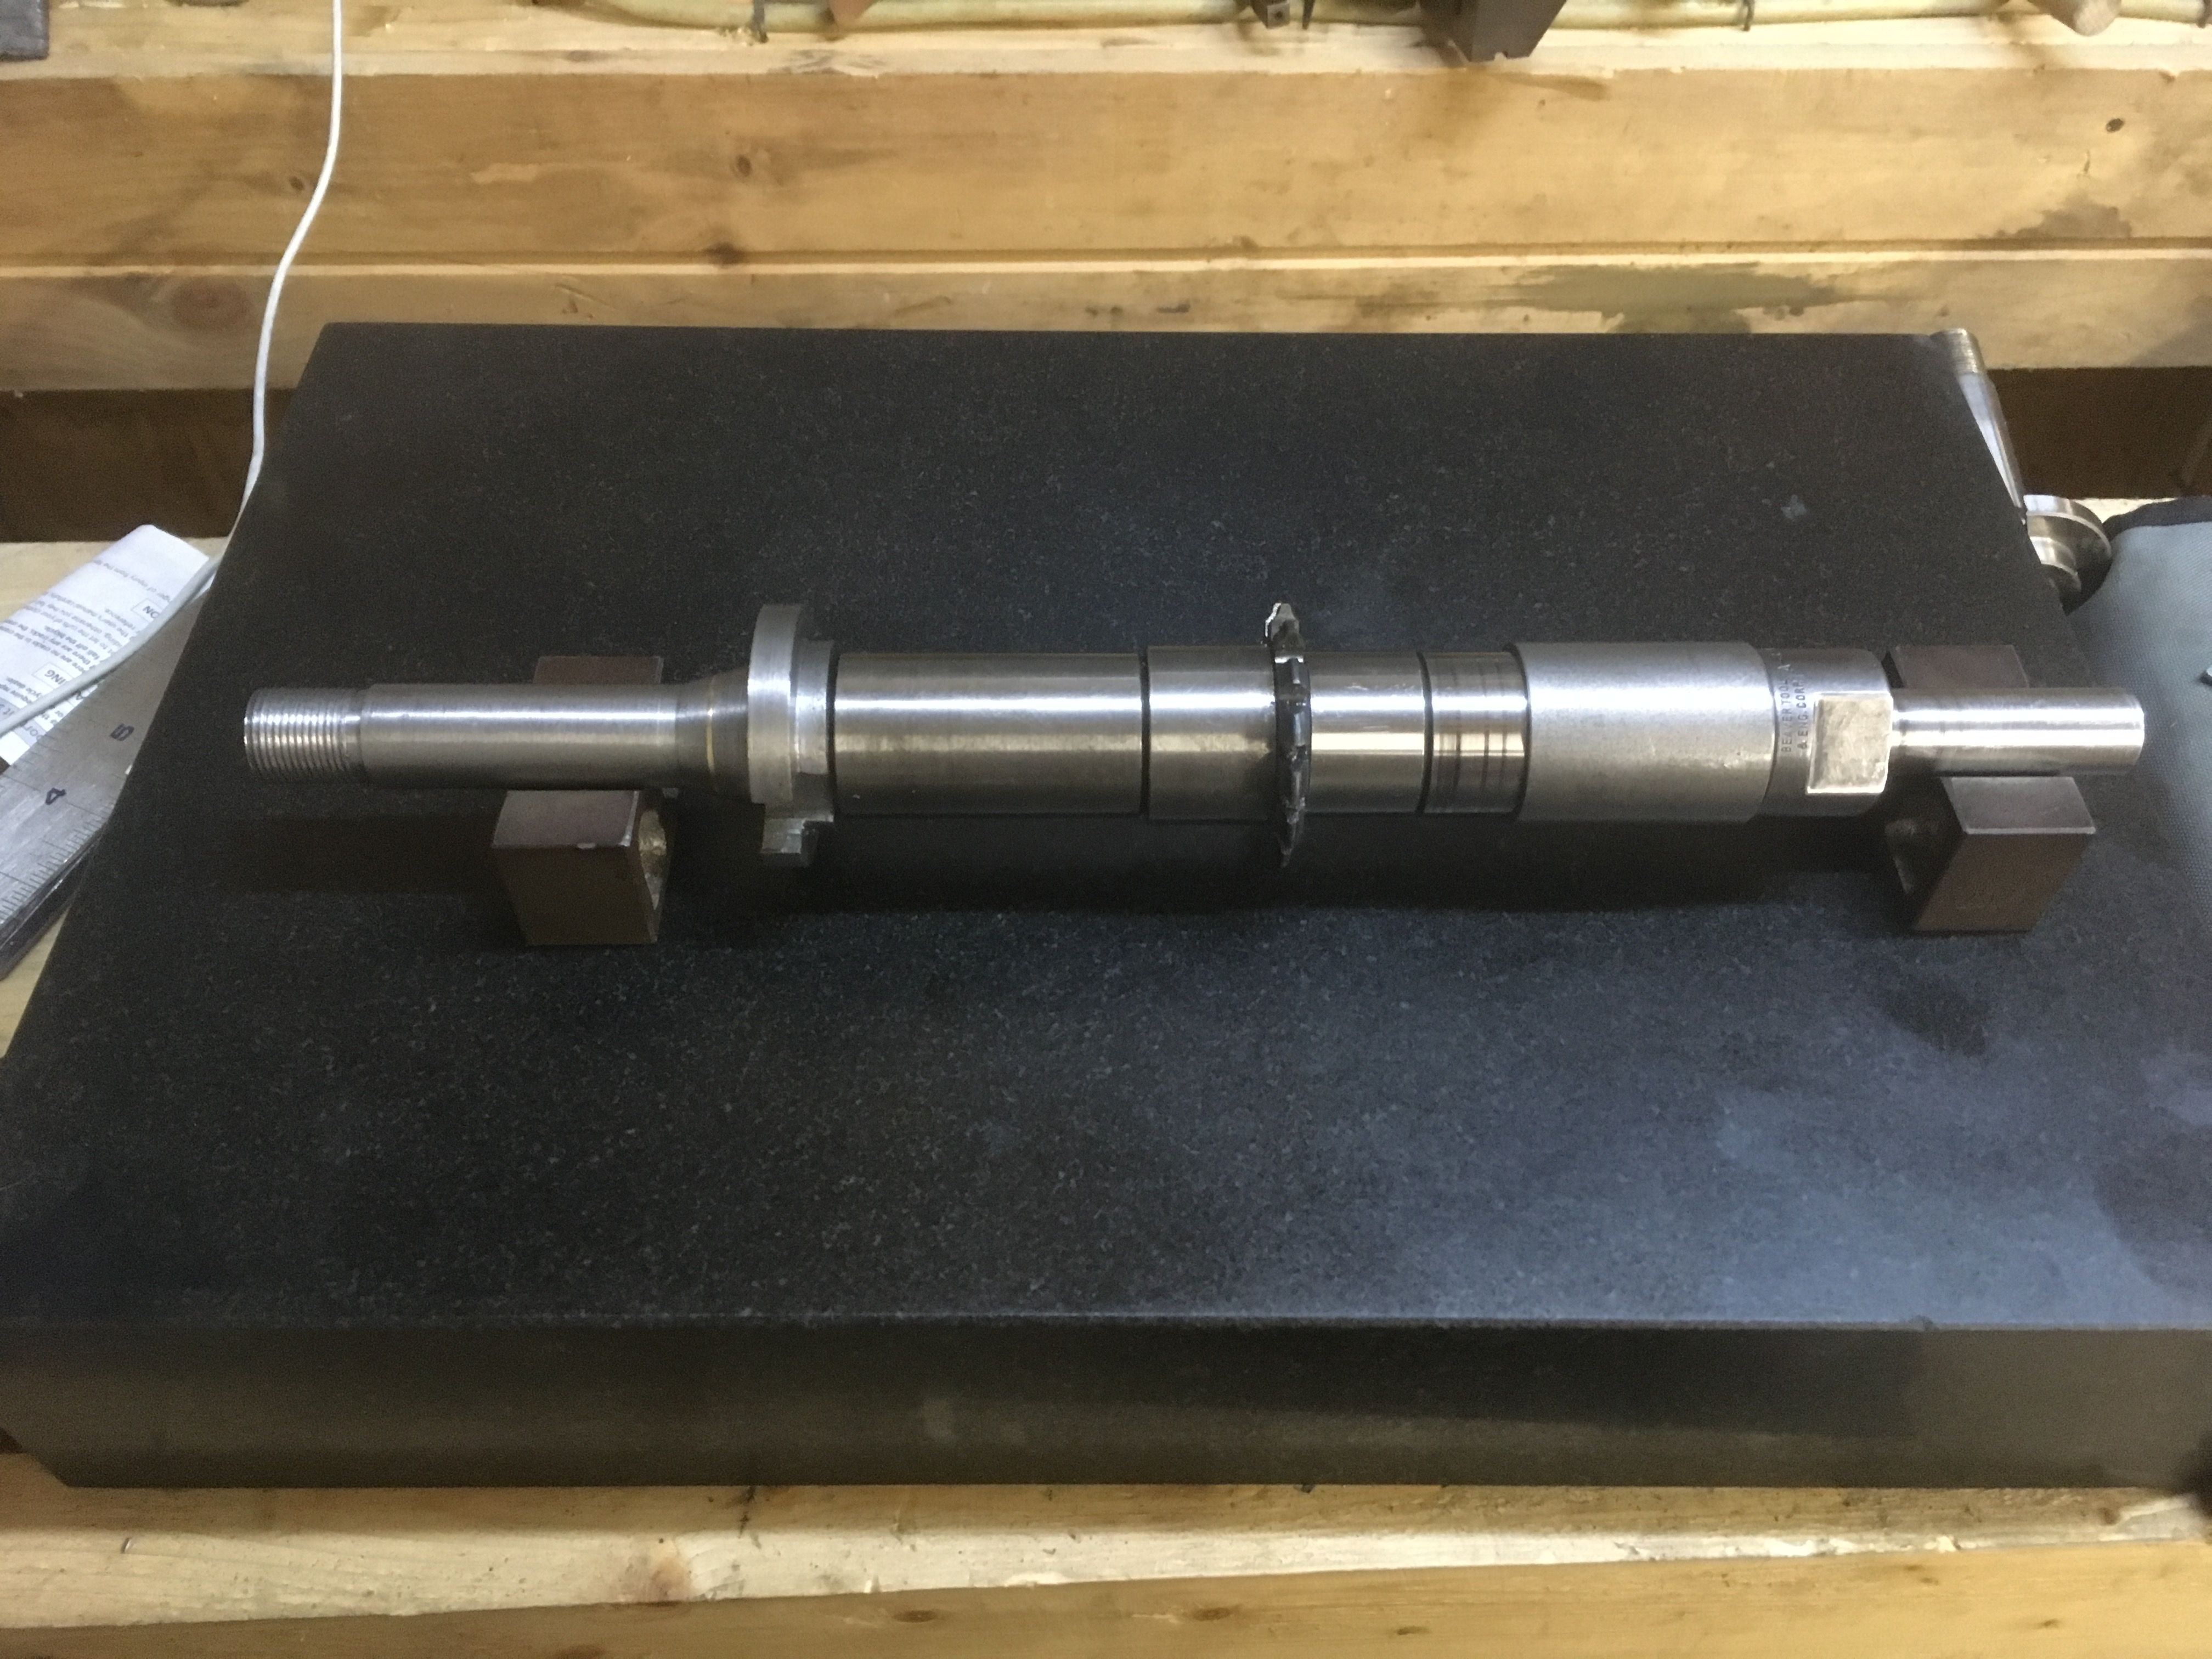
\includegraphics[width=5in]{cutterArbor}
	\caption{Cutting Arbor Setup. From left to right, you can see the part of the cutter arbor that mounts in the machine spindle, two spacers, the gear cutter itself, three more spacers, and the take-up nut.}
\end{figure}

\clearpage
\subsubsection{Choosing the Cutter}
The cutter is to be chosen based on the diametral pitch and the number of teeth to be cut. Once you have a set of cutters for your given diametral pitch, you will notice they are numbered:

\begin{figure}[H]
\centering
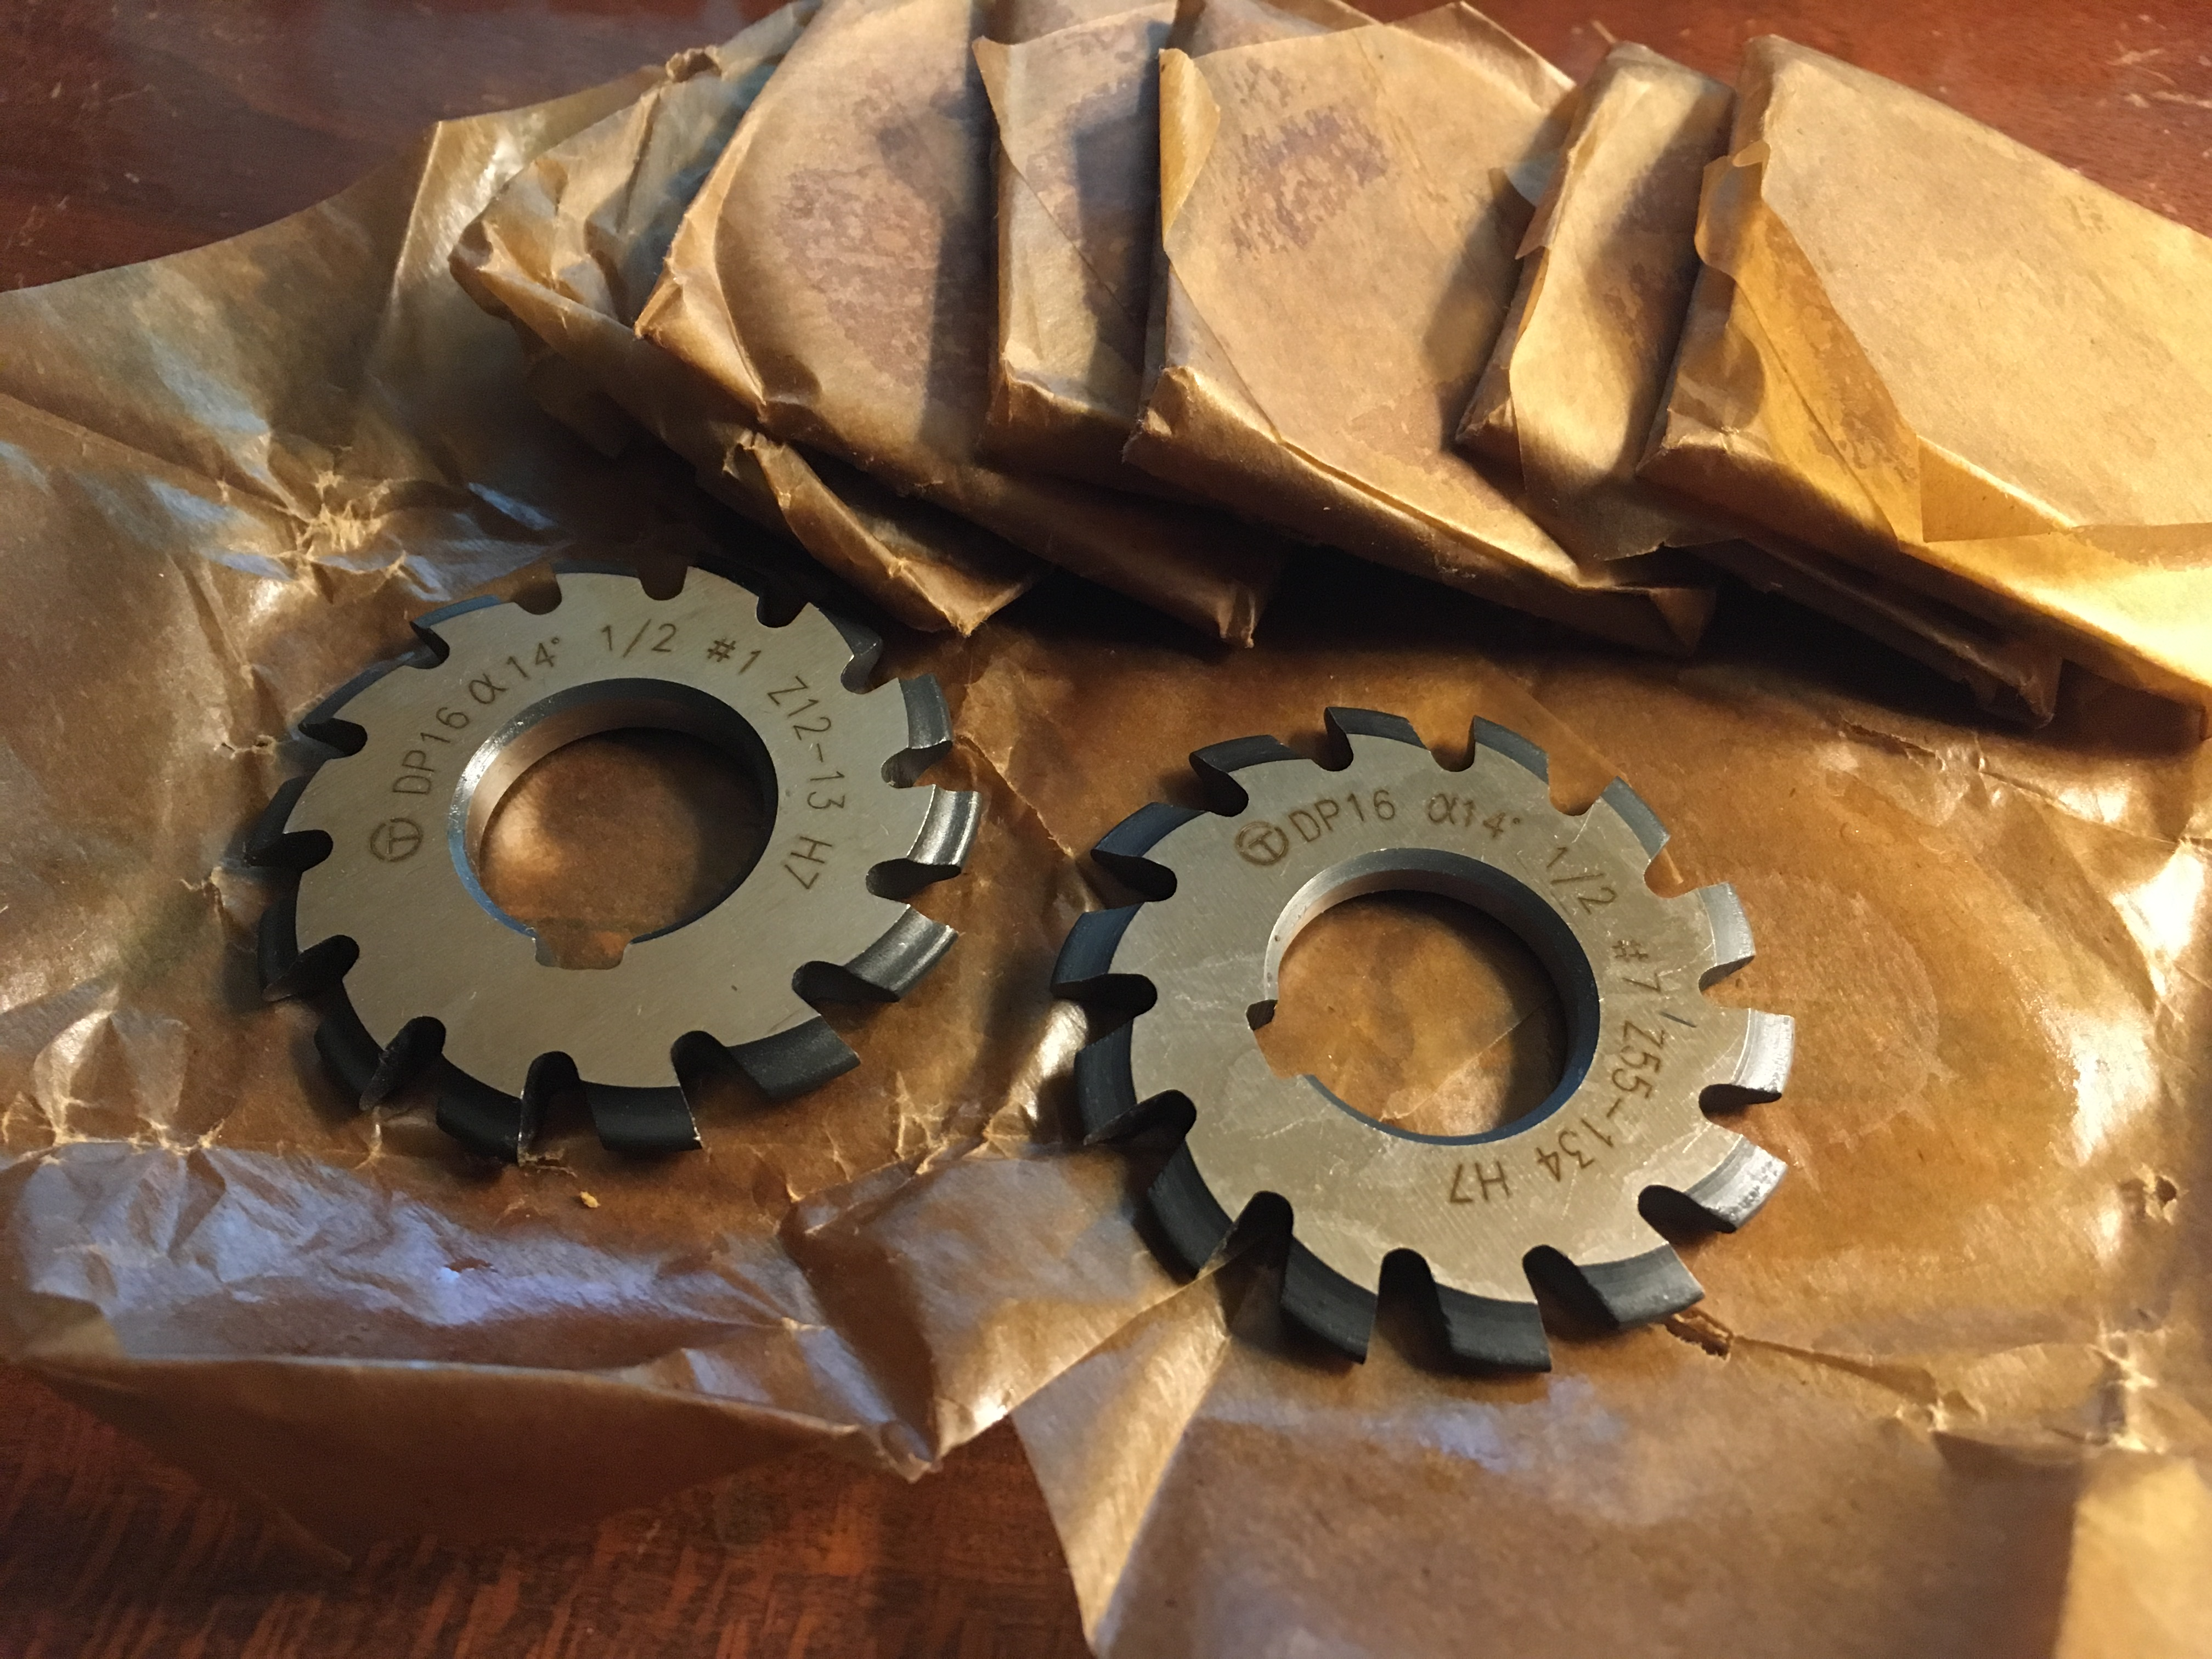
\includegraphics[width=5in]{cutter2}
	\caption{Series of Gear Cutters, for 16dp.}
\end{figure}

In the case of the example 24-tooth gear, I chose a number 5 cutter, because it is labeled ``DP16 $\alpha$ 14 1/2 Z21-25'', indicating it can cut 16 diametral pitch gears with a 14.5 degree pressure angle, and anywhere between 21 to 25 teeth. The $\alpha$ stands for ``angle,'' and the Z for teeth (from German ``Zahn,'' or tooth.)

\clearpage
\subsubsection{Assembling the Cutter Arbor}

\begin{enumerate}
	\item Place the key in the keyway of the cutter arbor, if keyed drive is desired. Gear cutters are small enough that friction-drive alone can often make them work with a sufficiently tight assembly.
	\item Place spacers on the cutter arbor until about half the space is taken up.
	\item Place the cutter on the arbor.
	\item Put the rest of the spacers on the arbor, ensuring that the spacers protrude into the threaded area of the arbor.
	\item Screw the nut onto the end of the arbor, and tighten it onto the spacers.
	\item Place the cutter arbor in the machine, ensuring that it fits properly into the spindle taper.
	\item Screw the drawbar into the rear threads of the arbor, and tighten it.
	\item Loosen the arm binders for the round overarm support bar.
	\item Move the arbor support and the round overarm support bar, so that the end of the arbor rests in the bearing hole of the support.
	\item Tighten the arm binders.
	\item Turn the spindle by hand using the spindle handwheel to ensure the setup works smoothly before applying power. 
\end{enumerate}

\subsection{Speeds and Feeds}
\begin{figure}[H]
\centering
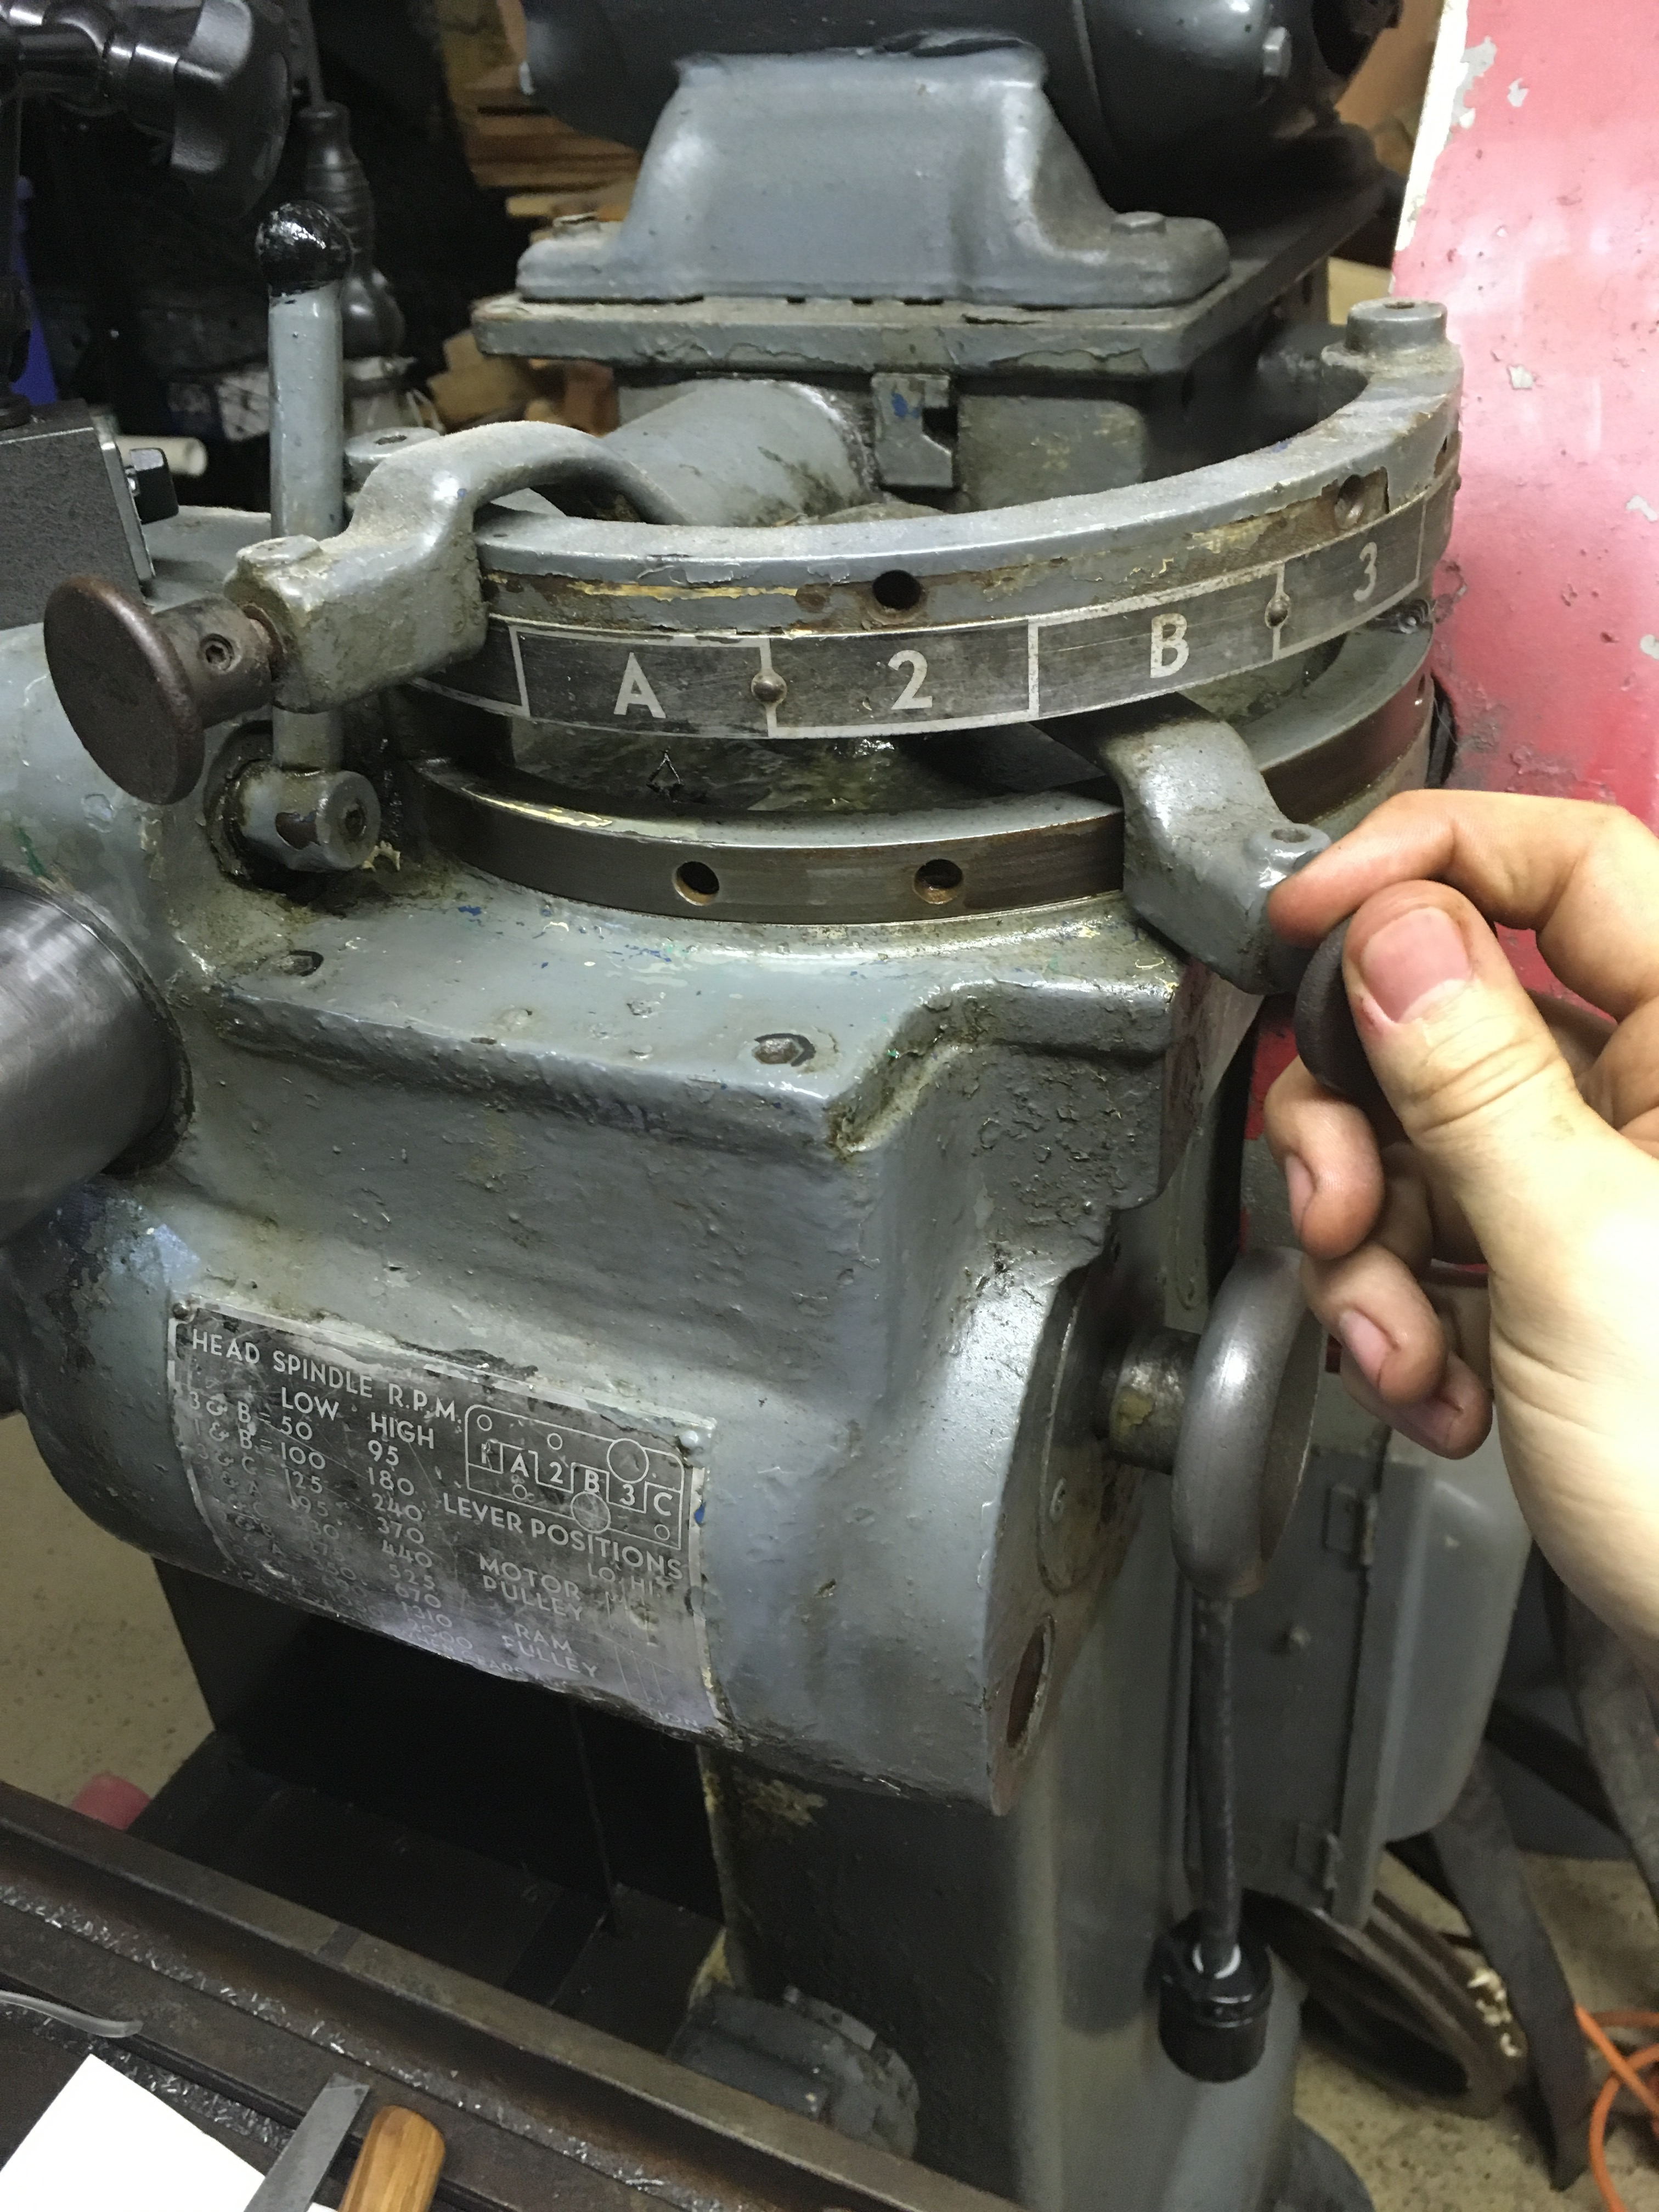
\includegraphics[width=5in]{speedSetting}
\caption{The spindle speed settings on the machine. Note the table in the bottom left - this will show the operator how to translate spindle speed into the appropriate lever positions.}
\end{figure}

\subsubsection{Calculating the Ideal Speed and Feed}

Speeds and feeds are vital parameters in milling operations. ``Speed'' refers to the spindle speed in RPM, and ``feed'' refers to the feed rate of the work into the cutter, generally given in ipm or inches per minute. Speed is calculated backwards from cutter diameter, as the ultimate parameter being controlled is the surface speed of the cutting edge, which is faster for a larger cutter at a given number of RPMs.

In our case, we have a cutter of 2.2 inches outer diameter, and according to machinery's handbook, we should be looking for between 50 to 100sfm (Horton, 1954, p. 1503), or surface feet per minute. To determine the speed in sfm, `S', of the outside of a cutter with diameter `D' at a level of rpm 'R', we can employ this formula:


	\[S \;sfm = \frac{\pi \times D \; in \times R \;rpm}{12 \; in/ft}\]

If we need to find the rotational speed instead, we rearrange the equation:

	\[R\; rpm= \frac{12 \times S \;sfm}{\pi \times D \;in}\]

So for a 2.2 inch cutter at the lower 50 spm speed, we have:

	\[86.81 \; rpm = \frac{12\;  in/ft \times 50\;  sfm }{\pi \times 2.2\;  in} \]

Doing the same thing with 100 rpm, we get 173.62 rpm, so the spindle speed should be somewhere between 86.81 and 173.62 rpm for a 2.2 inch OD gear cutter. 

Feed rates have more to do with how much material is removed by each tooth of the cutter, a property called chip load. In the example case, our gear cutters have 14 teeth and are spinning at 100 rpm. This yields 1400 teeth contacting the material per minute. For a \textbf{chip load} of .005 per tooth, a common, modest chip load, we would multiply the teeth per minute by the load per tooth to get the total inches per minute of feed. This yields:
\[ 1400 teeth/min \times .005 in/tooth = 7 ipm \]

So the feed would be something like 7 ipm, which is one of the options available on the speed selector. Both arms of the speed selector on the knee of the mill should be moved over a section that has ``7'' written on it in order to select that speed.



\subsubsection{Setting up the Mill for Speed and Feed}
\begin{figure}[H]
\centering
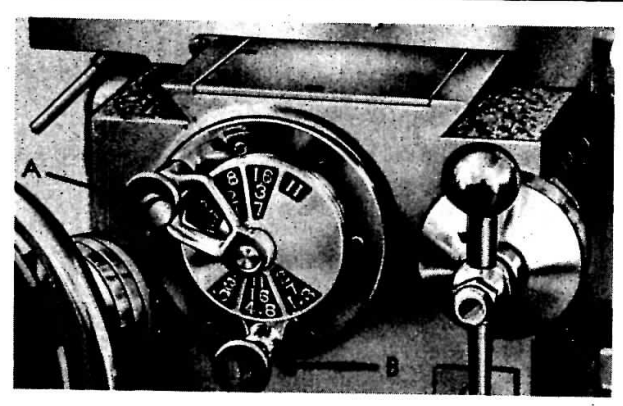
\includegraphics[width=5in]{feedSelect}
	\caption{Feed Selector for Van Norman 16 mill. Adapted from ``Installation, Operation, and Maintenance Instructions and Parts List for No. 16 Van Norman Ram Type Milling Machine Plain and Universal Models'' [Pamphlet]. (1952). Springfield, MA: Van Norman Company. }
\end{figure}
\begin{enumerate}
	\item Use the speed chart on the head of the mill to select the range corresponding to what was determined in the previous section. I chose 100rpm, or setting 1B, for the example gear, as it falls in the lower end of the acceptable speed range.
	\item Select the appropriate feed range using the levers of the speed selector. Both levers should fall over the range of the speed that is desired - for 7ipm, for instance, both of the windows of the levers should fall over a wedge with ``7'' written on it.
\end{enumerate}

\subsection{Centering and Zeroing the Cutter}

\begin{figure}[H]
\centering
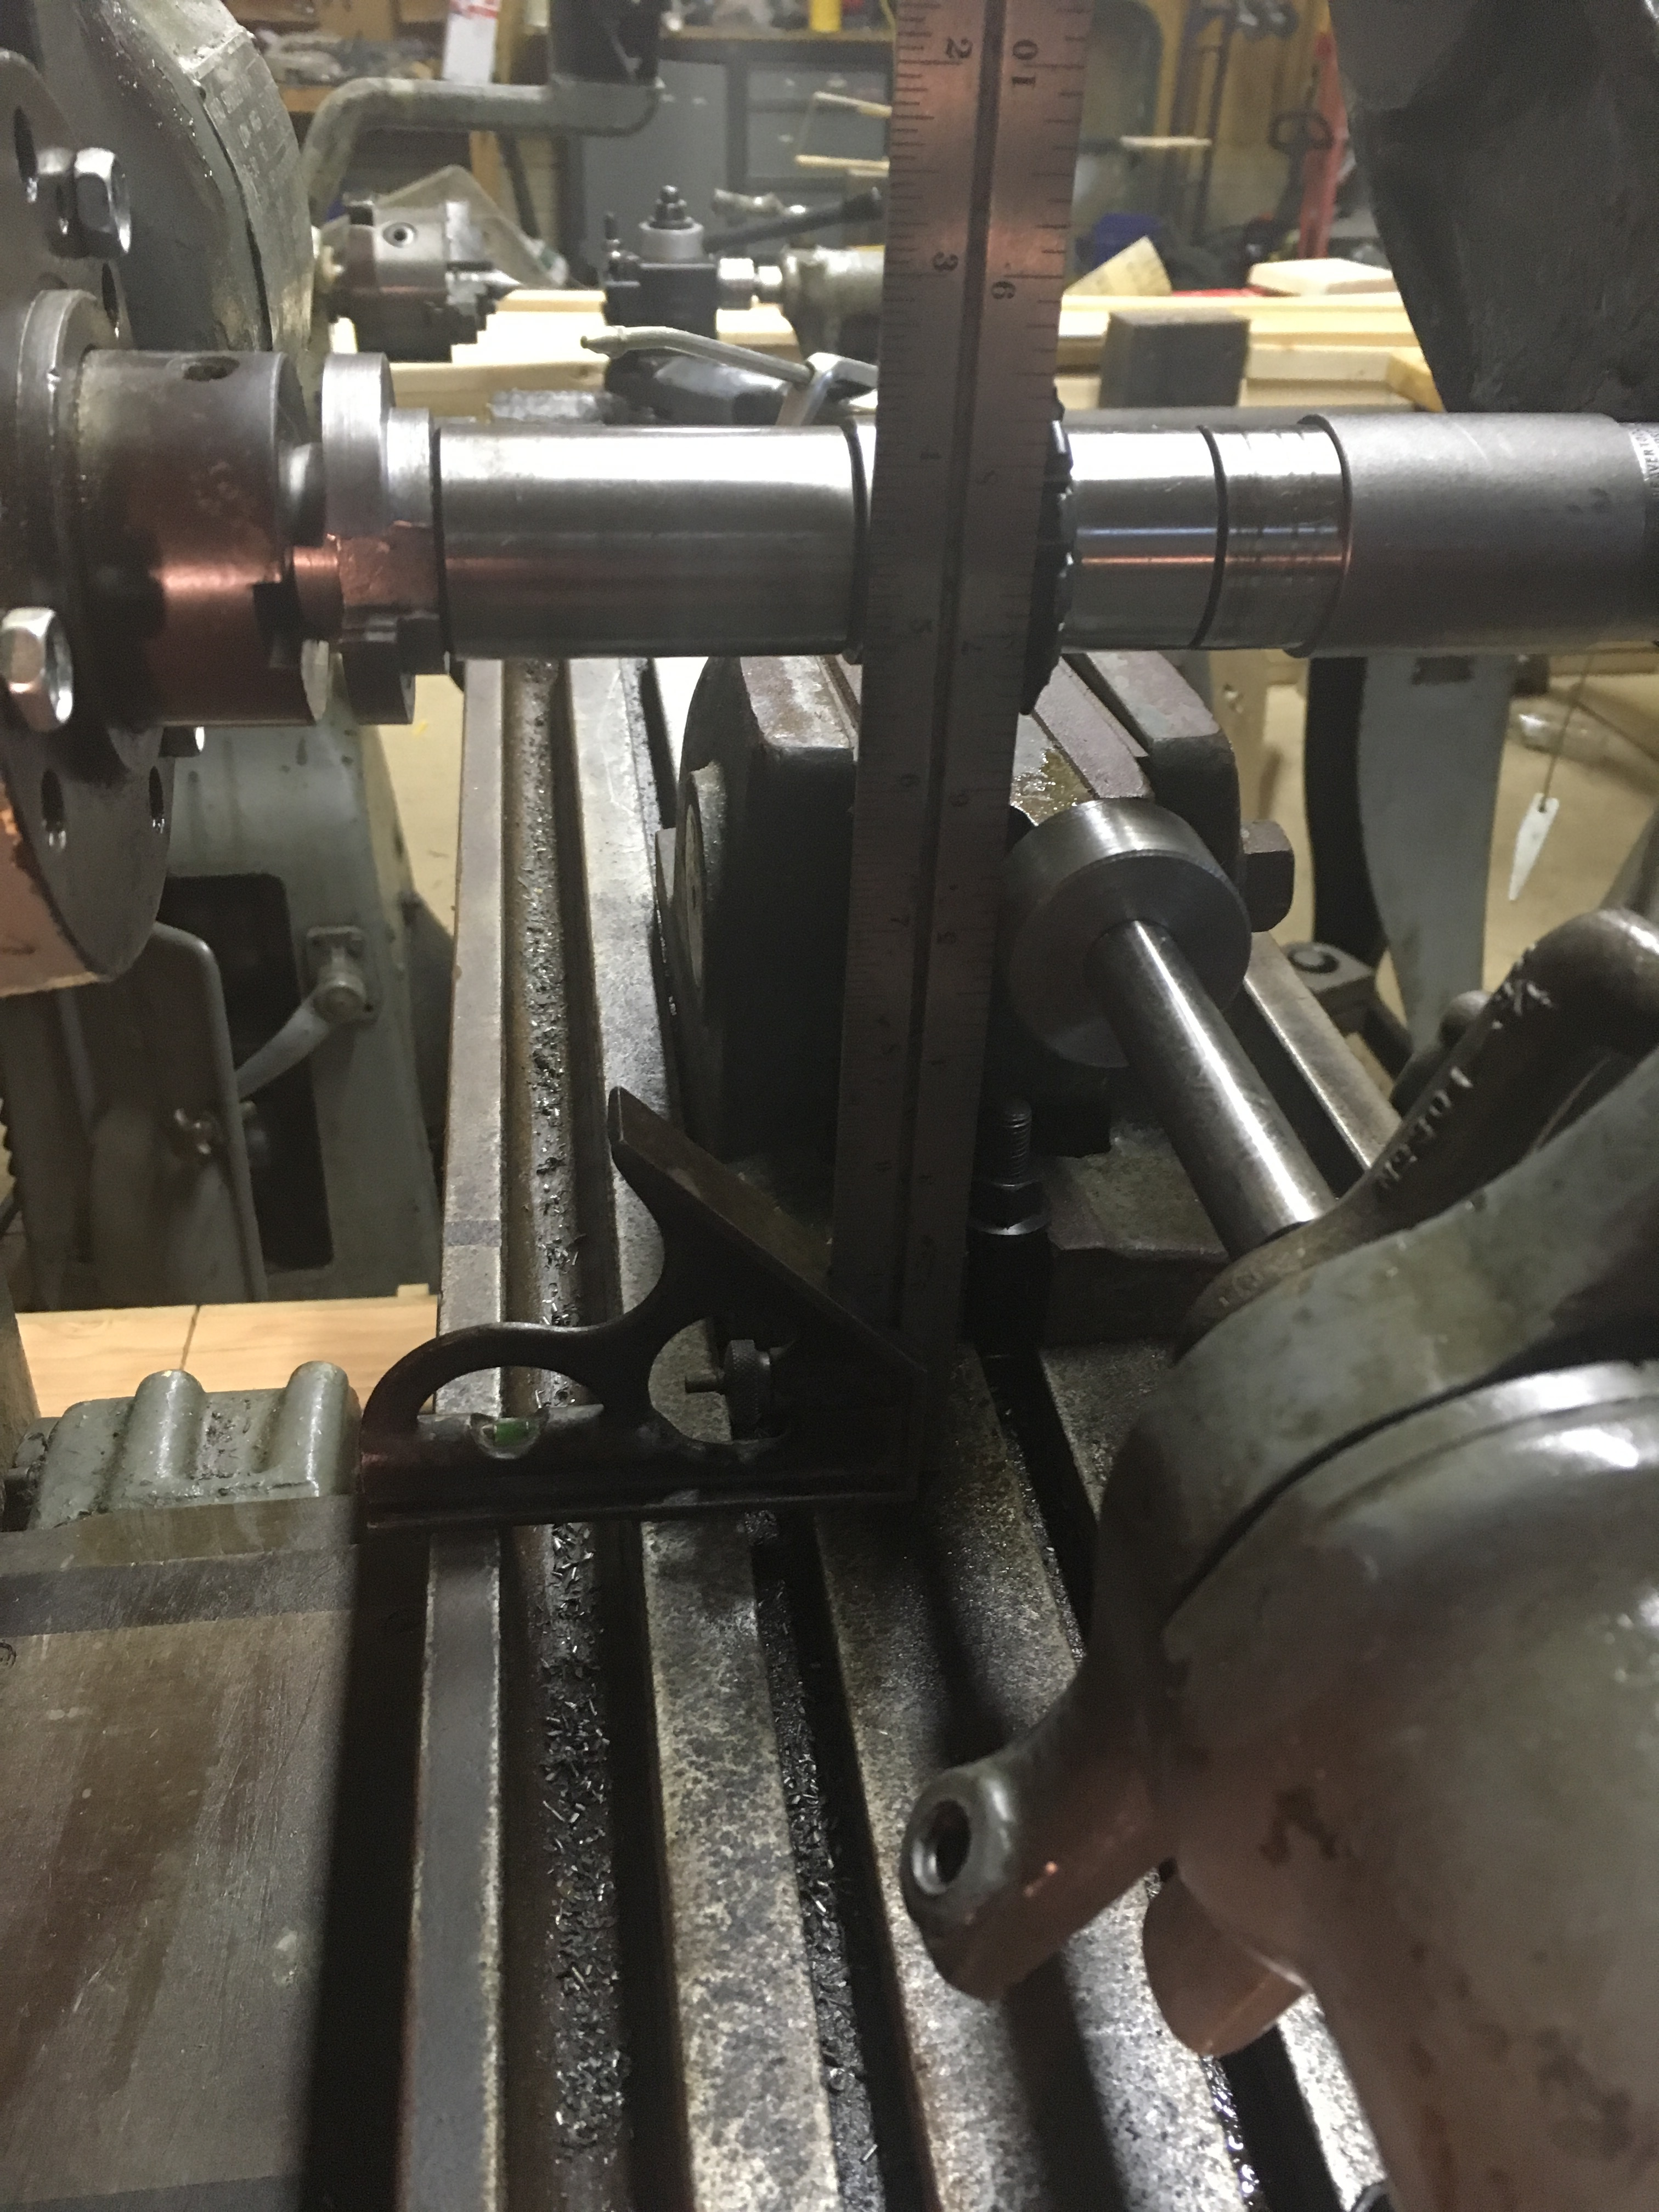
\includegraphics[width=5in]{blankAlign}
	\caption{Aligning the cutter and the gear blank using a machinist's square.}
	\label{fig:cutterAlign}
\end{figure}


	There are a number of methods for centering the milling cutter, but we will choose one requiring a minimum of measuring tools. It is ideal to do this with an indicator or a DRO, and it is generally frowned upon to use the dials for direct measurement. Nevertheless, here is a procedure for doing just that, in case another means of centering is not available:

\begin{enumerate}
	\item Using the square on the mill table, align the rear edge of the cutter with the corresponding rear point on the edge of the gear blank (see Figure \ref{fig:cutterAlign}.)
\item Find the offset W using cutter thickness T and gear blank diameter D: \[ W = \frac{1}{2} T \times D\]
\item Crank the table cross feed back by the dimension calculated.
\item Engage the saddle binder.
\item Center the part longitudinally, by eye only, using the table handwheel.
\item Start the spindle.
\item Raise the table to the cutter using the vertical feed handwheel until the cutter just touches off the top of the blank. It should barely scratch the surface. 
\item Stop the machine using the 'stop' button.
\item Engage knee binder.
\item Set the vertical feed collar to zero.
\item Disengage knee binder.
\item Feed the table to the right so that the cutter is past the gear blank, but still over the mandrel.
\item Raise knee by calculated whole depth of tooth cut, $h_t$. 
\item Engage knee binder.
\item Loosen the vertical feed collar and set the dial to zero. 
\item Disengage knee binder.

\end{enumerate}

\begin{figure}[H]
\centering
	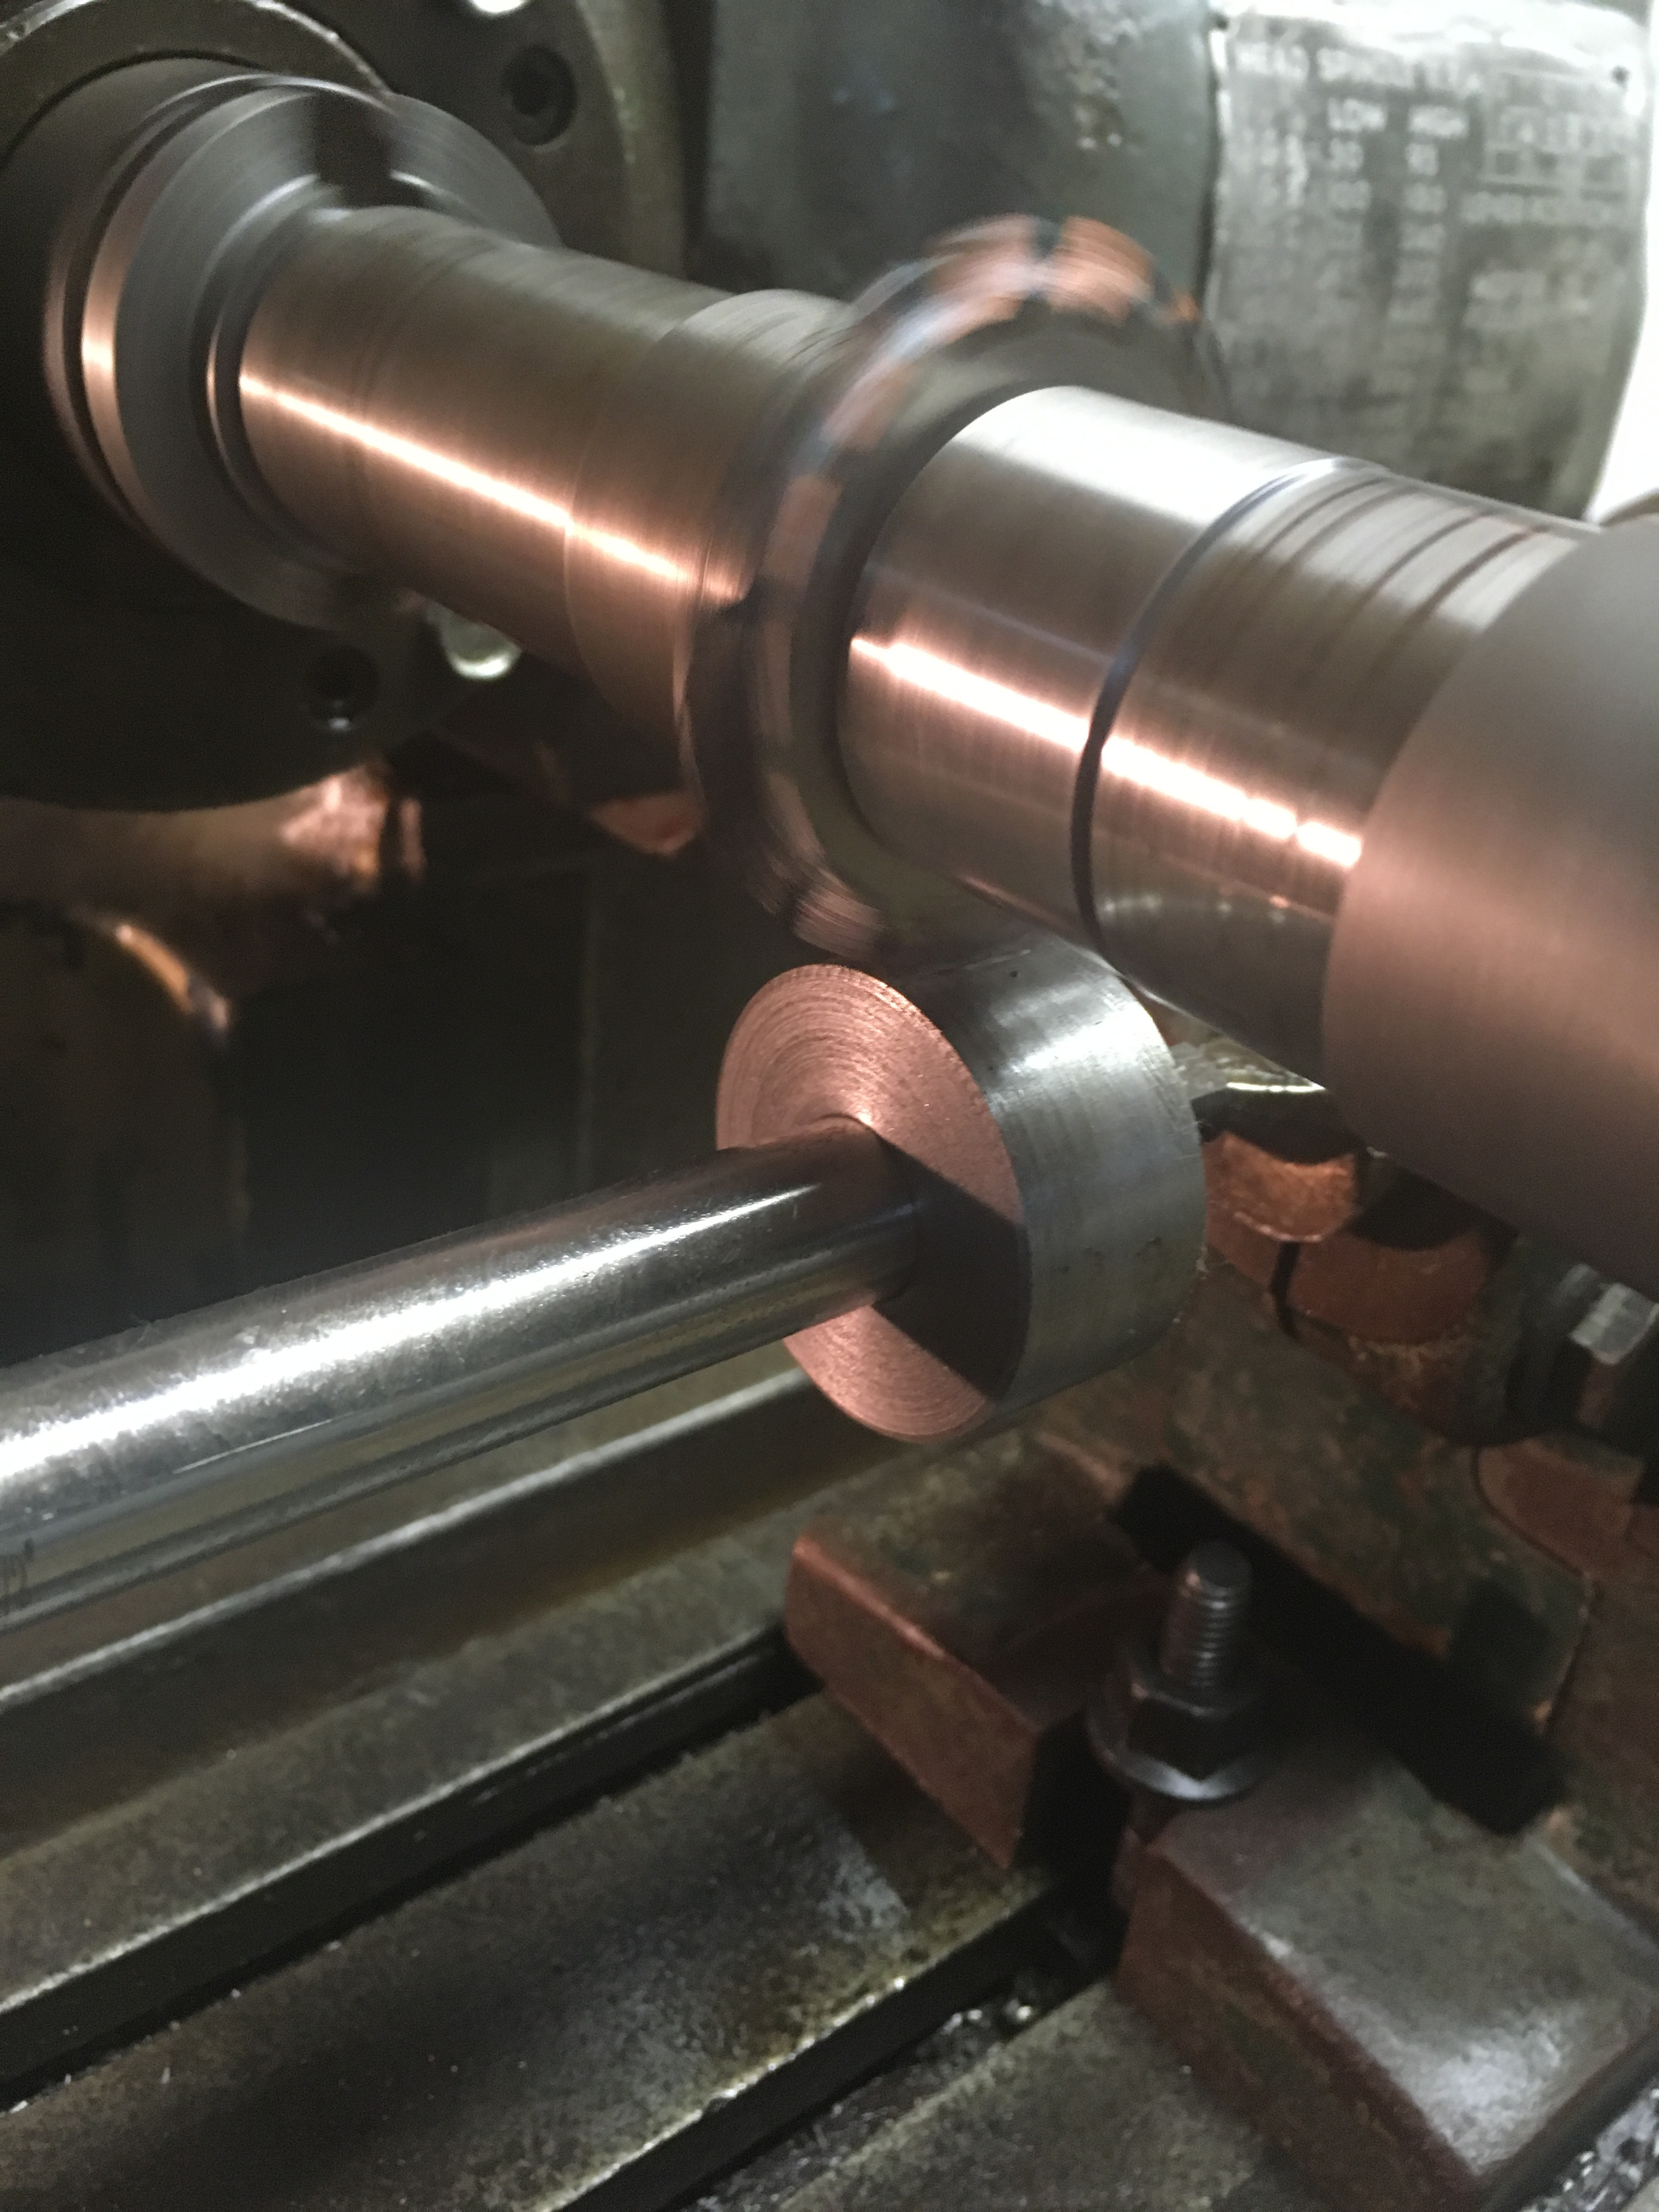
\includegraphics[width=4.5in]{touchOff}
	\caption{Touching off on the top of the gear blank. Notice how the cutter has barely scratched the surface of the blank.}
\end{figure}



\section{Gear Cutting}
In this section, we cover the operation of the milling machin in actuall producing the tooth profile of the gear we have been preparing for. 
\begin{figure}[H]
	\centering
		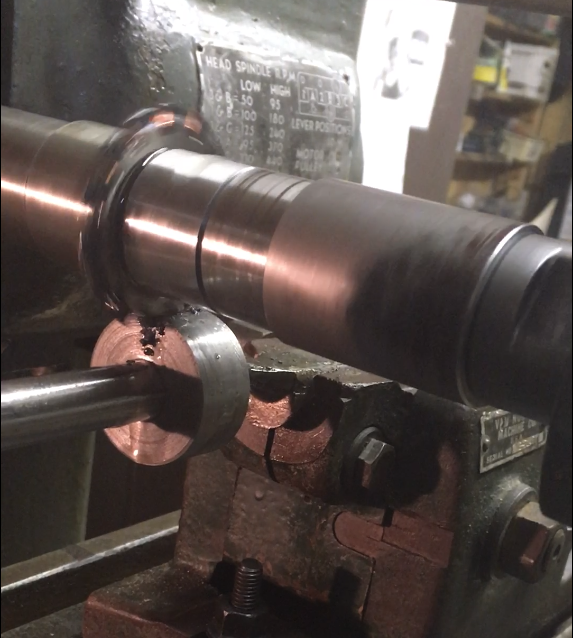
\includegraphics[width=5in]{firstCut}
	\caption{Cutting the first tooth.}
\end{figure}

\clearpage
\subsection{First Cut and finding the Zero Point}
\begin{enumerate}
\item Apply lubricant or engage cutting fluid pump.
\item Start spindle and automatic feed motor.
\item Engage table power feed lever.
\item When the cutter has passed the work and is no longer cutting, disengage feed lever.
\item Stop spindle, table motor, and coolant.
\item Use table hand wheel to feed work out from under spindle, far enough to access with measuring tools. Ensure that the spindle is stopped.
\item While in machine, measure cut using one gear wire and the back end of the gear blank. Use Machinery's Handbook to reference necessary dimensions.
\item Determine how far off the measurement is from the ideal measurement. Adjust the vertical feed by the amount that the measurement is off, and re-zero handwheel, binding the vertical feed before zeroing and releasing it immmediately afterwards.

\item Lower the vertical feed by .200.
\item Return the table to pre-cut position by hand wheel.
\item Raise the vertical feed by .200, back to new zero point.

\item Engage the spindle, coolant, and table feed and re-cut gear to reach target dimension.
\item Stop spindle, feed, and coolant.
\item Move table out to measuring position again, and re-measure gear. If it has not reached the proper dimension, re-adjust and repeat the foregoing steps until it has.

\item Lower the table by .200 and return to pre-cut position.
\end{enumerate}

\subsection{Cutting the Rest of the Teeth}
\begin{figure}[H]
	\centering
		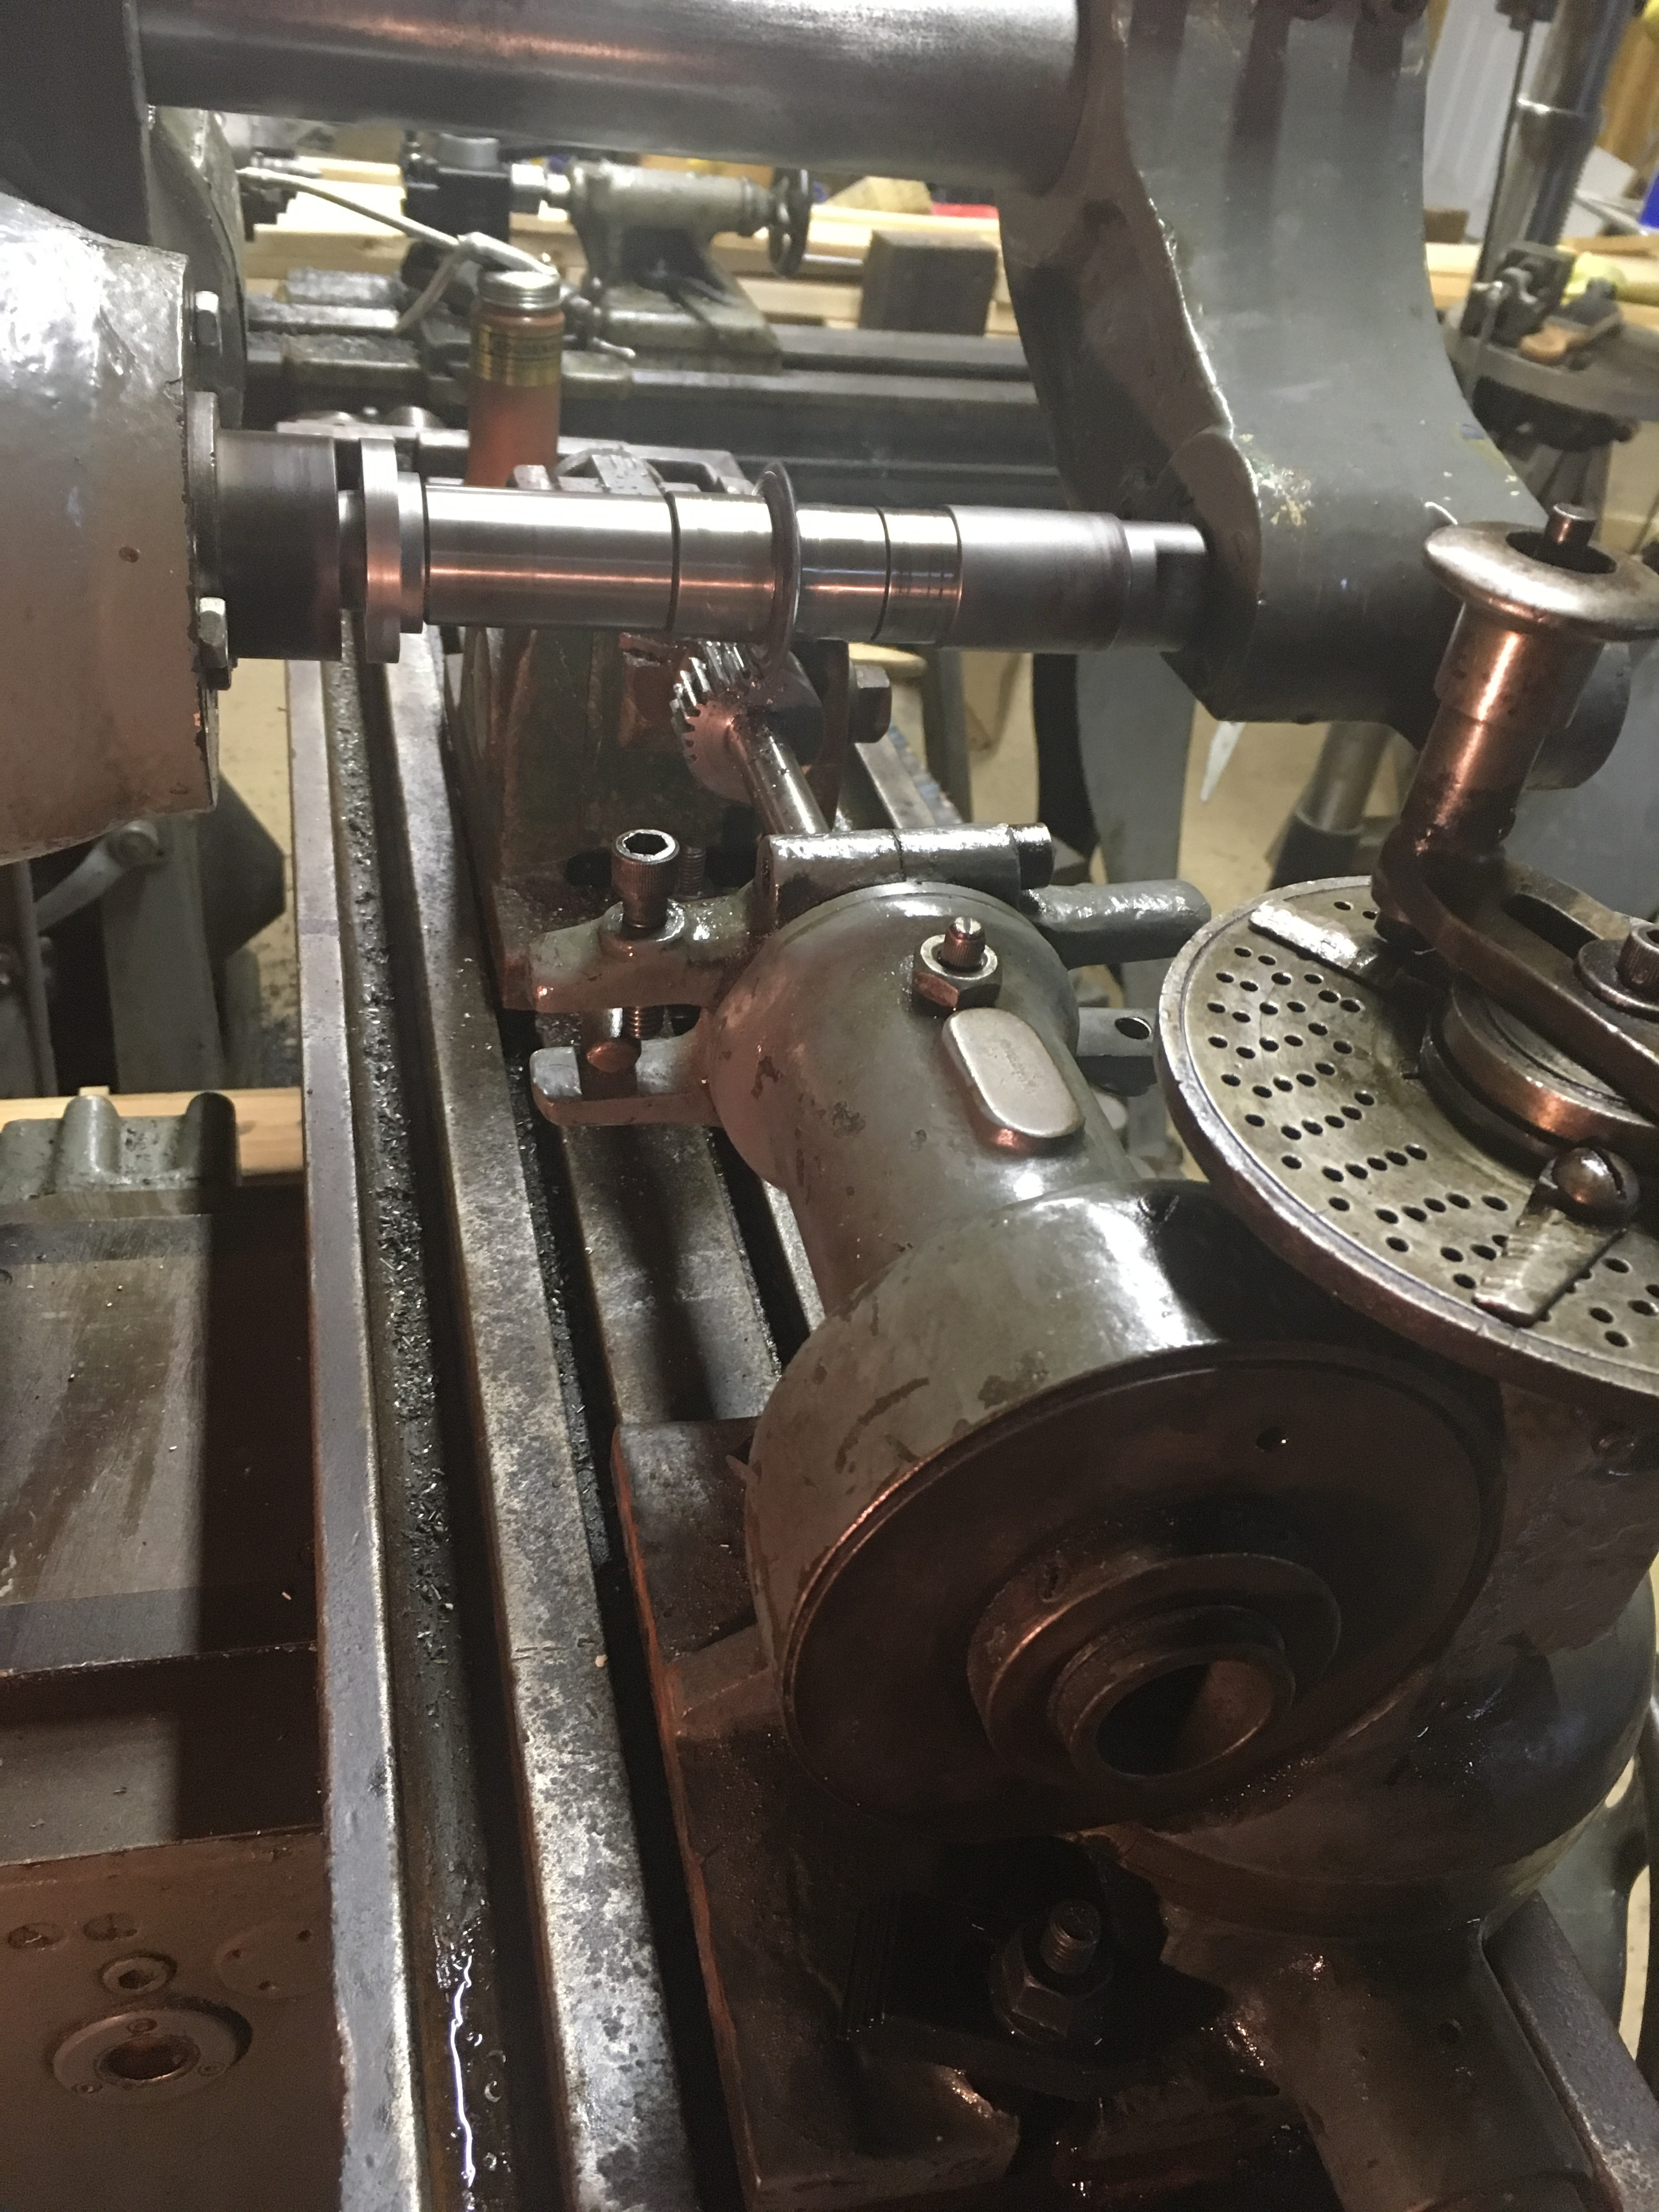
\includegraphics[width=5in]{midProcess}
	\caption{A 24-tooth, 16dp gear being cut - this one is several teeth into the cutting process.}
\end{figure}
The rest of the cuts are where the routine work sets in. Each gap in small gear is cut individually at full depth, and the gear is rotated using the index between cuts. 
\begin{enumerate}
\item Ensure that the sector arms of the index and the pin are in the correct places as per the setup section.
\item Place the rear of the sector arm just counterclockwise of the index pin.
\item Lift the detent on the worm gear arm on the index, and rotate it clockwise by the calculated number of turns, plus the remainder indicated by the sector arms.
\item Rotate the sector arms until they are touching just counterclockwise of the index pin.
\item Apply cutting fluid if not working with a coolant system.
\item Engage the automatic table feed,  and wait for cut to complete. Disengage table feed using feed lever.
\item Disengage the knee binder.
\item Drop the vertical feed by .200.
\item Feed table by hand to reach starting position.
\item Raise the vertical feed by .200.
\item Engage the knee binder.
\item Are all teeth cut? If not, return to step 1. Otherwise, continue on to verifying the measurements of the gear.
\end{enumerate}

\section{Verifying Measurements and Cleanup}

\begin{figure}[H]
	\centering
		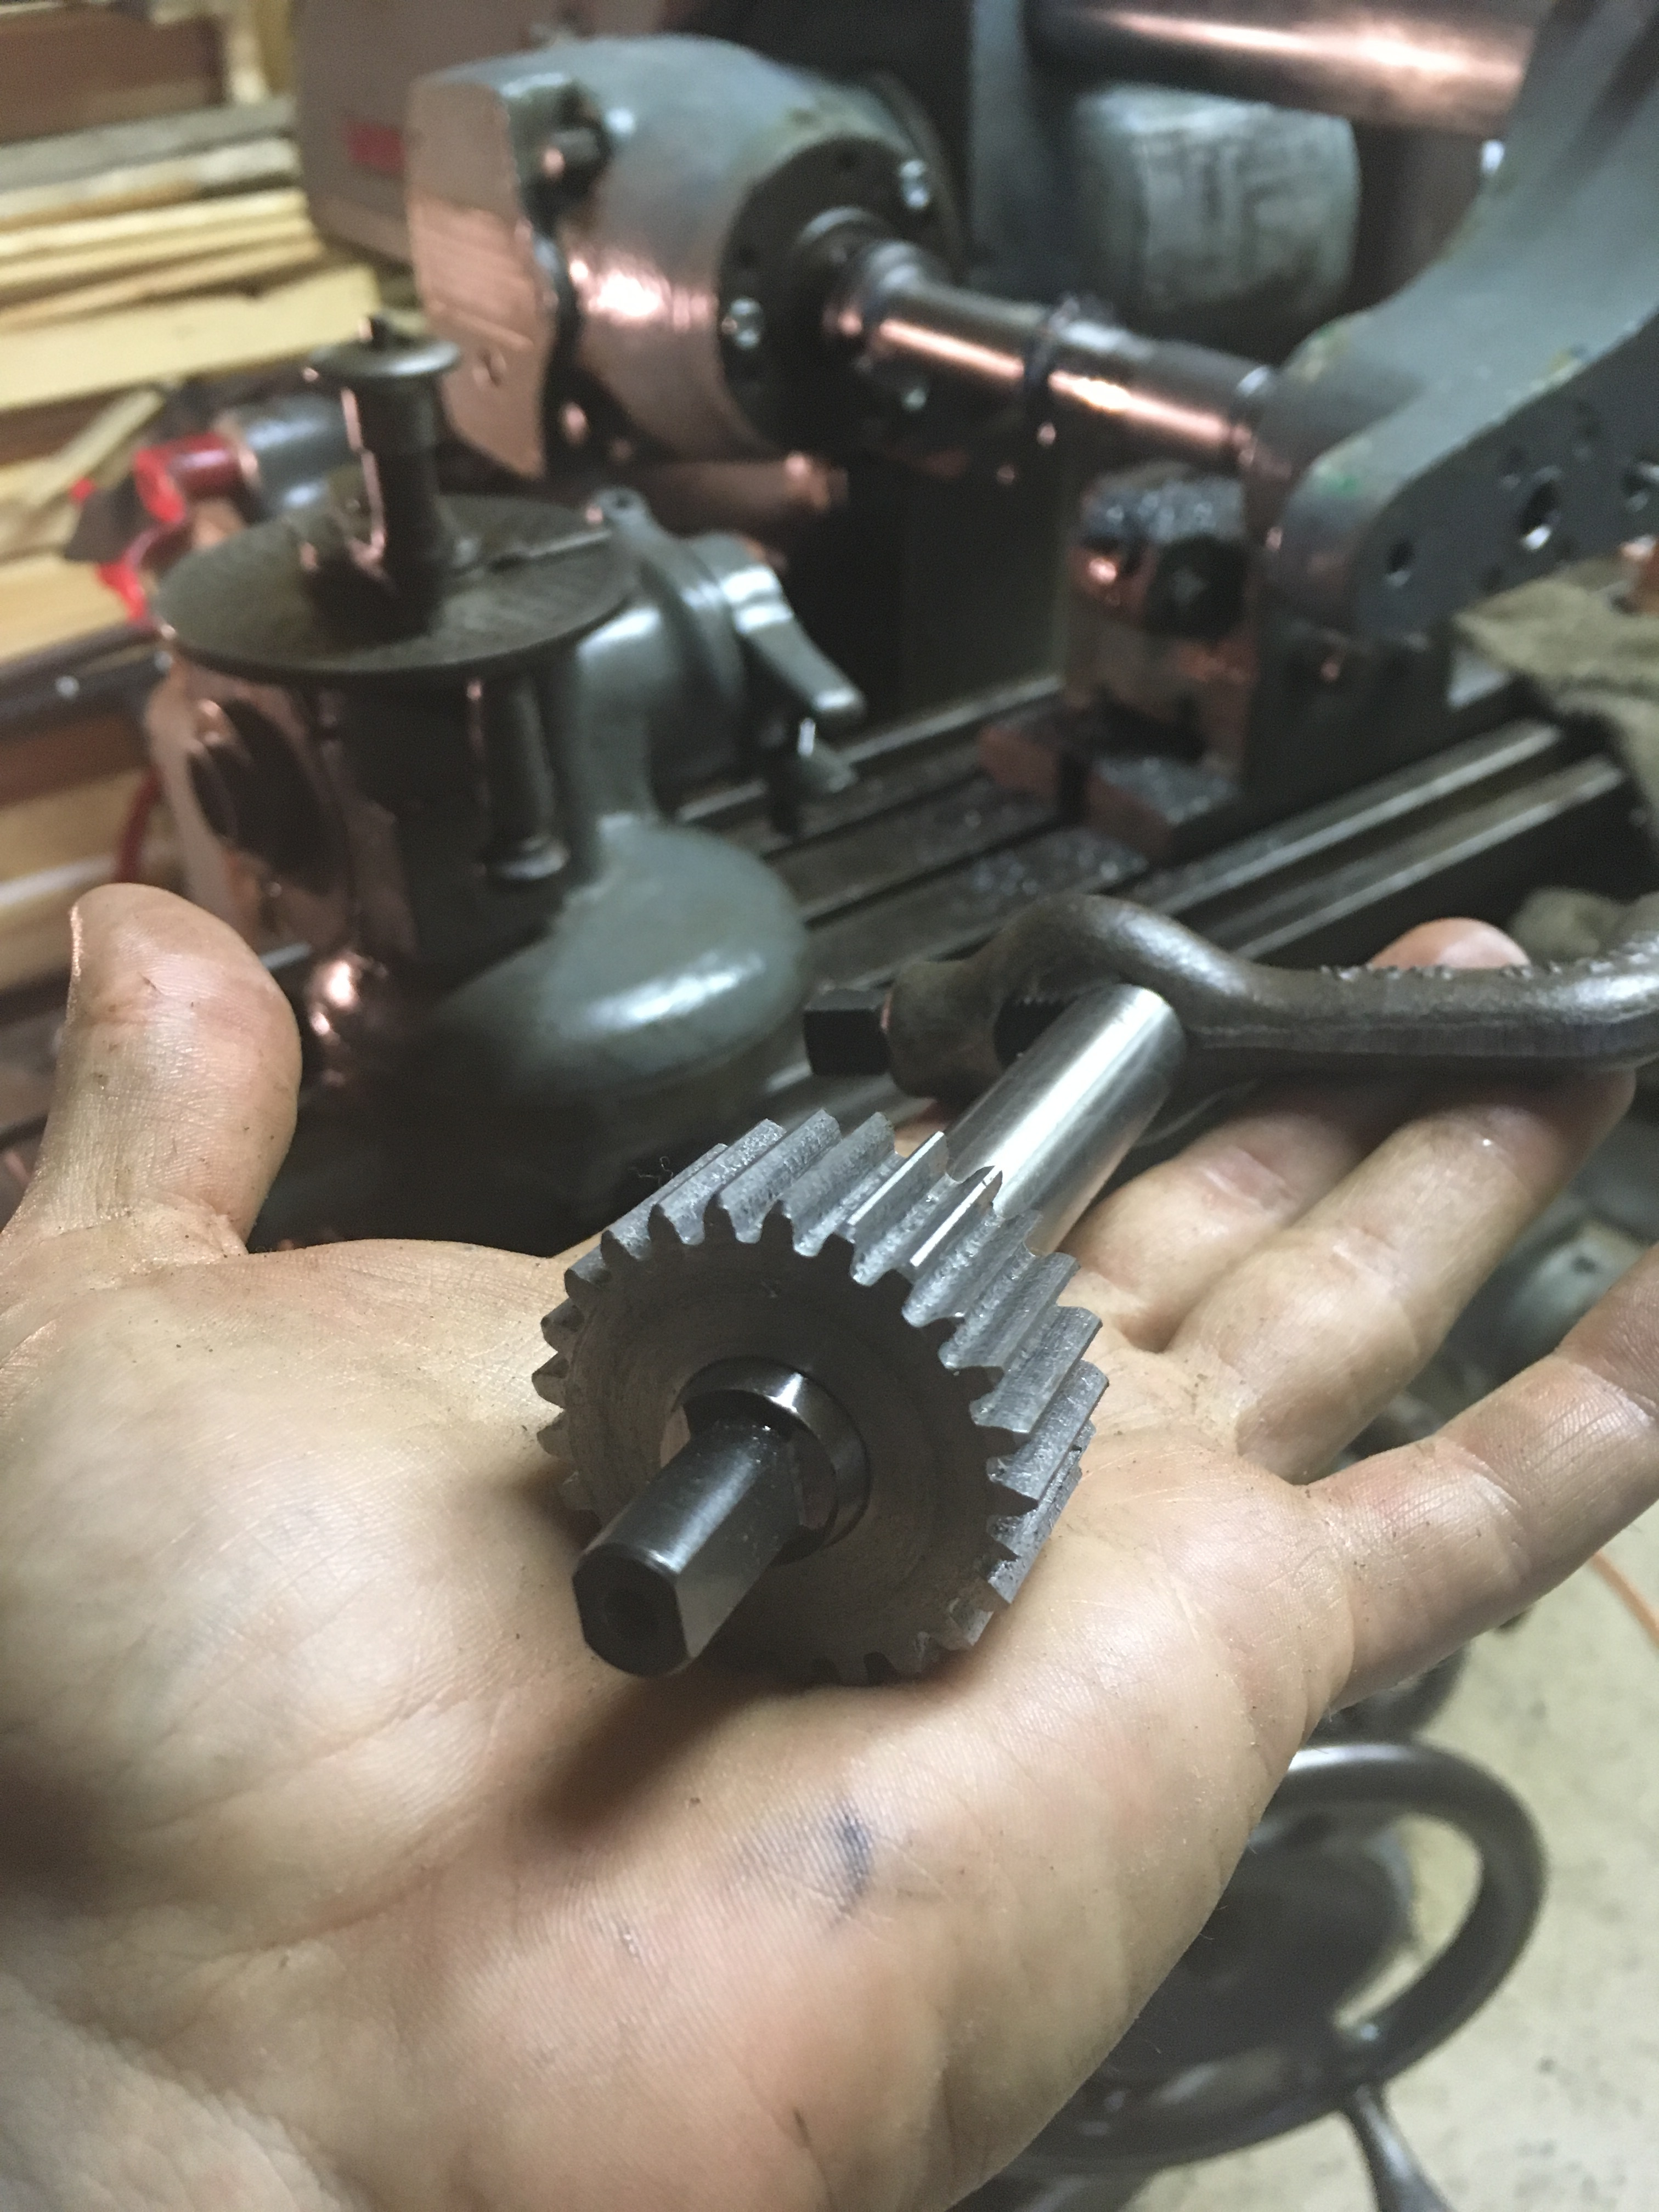
\includegraphics[width=5in]{finalProduct}
	\caption{A gear made on the VN16 mill. This one hand a hole-count error when using the index, resulting in two undersized teeth - consistent operation is important!}
\end{figure}
\subsection{Checking Measurements}
\begin{enumerate}
\item Stop the mill spindle.
\item Using table feed, move gear blank out from under the spindle.
\item With gear still on mandrel, measure gear across wires using the micrometer.
\item With any luck, the gear should be the correct size. If it is too large, you can go back and take off a few thousandths by repeating the same procedure with the table raised by half the error (that is, if it is .004 too big, raise the table .002, because we cut on the radius. Don't cut off twice the error!) 
\item Once the gear is the appropriate size, remove it from the mill by unlocking the tailstock and unscrewing the center handle.
\item Dismount the gear from the mandrel using an arbor press. 
\end{enumerate}

\subsection{Deburring and Cleanup}
\begin{enumerate}
\item Place the gear in a vise and use fine files to deburr and chamfer the edges of the cut.
\item Be sure to clean up all chips and wipe down the machine after use. This ensures everything is ready for setting up the next job!

\end{enumerate}



\section{Bibliography}

\begin{itemize}
	\item Installation, Operation, and Maintenance Instructions and Parts List for No. 16 Van Norman Ram Type Milling Machine Plain and Universal Models'' [Pamphlet]. (1952). Springfield, MA: Van Norman Company. 

	\item Horton, H. L. (Ed.). (1954). Machinery's Handbook (15th ed.). New York, NY: The Industrial Press. 
	\item Suvo. (2010, February 27). How to Measure Pressure Angle of a Gear – Gear Pressure Angle, Gear Terminologies, Equations. Retrieved from https://www.brighthubengineering.com/machine-design/65216-how-to-measure-the-pressure-angle-of-a-physical-spur-gear/
	\item Engineer's Edge, llc. (n.d.). Inspection Methods for Spur Gears | Single Pin Measurement Method. Retrieved from https://www.engineersedge.com/
		gears/gear\_size\_inspection.htm 

\end{itemize}

\end{document}
